% !TeX spellcheck = en_US
% Appendices
\clearpage
\appendix
\pagenumbering{Roman}  % Change page numbering to Roman numerals
\setcounter{page}{1}   % Start numbering from I
\newpage
\counterwithin{figure}{section} % Setzt den Figure-Zähler auf Abschnitt-Ebene zurück
\counterwithin{table}{section} % Setzt den Figure-Zähler auf Abschnitt-Ebene zurück
\section{Appendix - Going Viral: Inflation Narratives and the Macroeconomy}\label{sec:Appendix}

\subsection{Supplementary Figures and Tables}\label{subsec:Supplements}

\begin{figure}[h]
	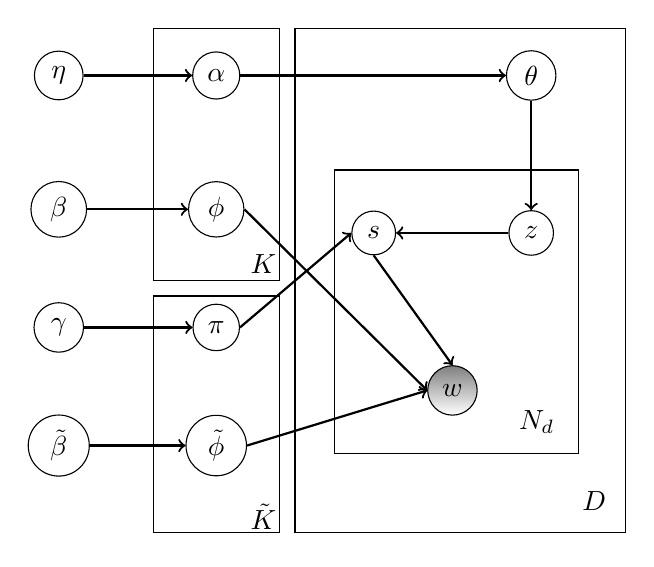
\begin{tikzpicture}
		%\node (p) at (-4,2) [circle,draw] {$\bm{P}$};
		%\node (htd) at (0,2) [circle,draw] {$h_{t[d]}$};
		\node (theta) at (0,0) [circle, draw] {$\theta$};
		\node (z) at (0,-2) [circle, draw] {$z$};
		\node (s) at (-2,-2) [circle, draw] {$s$};
		\node (a) at (-4,0) [circle, draw] {$\alpha$};
		\node (phi) at (-4,-1.7) [circle,draw] {$\phi$};
		\node (w) at (-1,-4) [shade,circle,draw] {$w$};
		\node (eta) at (-6,0) [circle,draw] {$\eta$};
		\node (beta) at (-6,-1.7) [circle,draw] {$\beta$};
		
		\node (gamma) at (-6,-3.2) [circle,draw] {$\gamma$};
		\node (pi) at (-4,-3.2) [circle,draw] {$\pi$};
		
		\node (tbeta) at (-6,-4.7) [circle,draw] {$\tilde{\beta}$};
		\node (tphi) at (-4,-4.7) [circle,draw] {$\tilde{\phi}$};
		
		
		%\draw[thick,->] (p.east) -- (htd.west);
		\draw[thick,->] (a.east) -- (theta.west);
		\draw[thick,->] (phi.east) -- (w.west);
		\draw[thick,->] (z.west) -- (s.east);
		\draw[thick,->] (s.south) -- (w.north);
		\draw[thick,->] (eta.east) -- (a.west);
		\draw[thick,->] (beta.east) -- (phi.west);
		%&\draw[thick,->] (htd.south) -- (theta.north);
		\draw[thick,->] (theta.south) -- (z.north);
		
		\draw[thick,->] (gamma.east) -- (pi.west);
		\draw[thick,->] (tbeta.east) -- (tphi.west);
		
		\draw[thick,->] (pi.east) -- (s.west);
		\draw[thick,->] (tphi.east) -- (w.west);
		
		\draw (-3,-5.8) rectangle (1.2,.6);
		\draw (-2.5,-4.8) rectangle (0.6,-1.2);
		\draw (-4.8,-2.6) rectangle (-3.2,.6);
		
		%\draw (-4.8,-2.6) rectangle (-3.2,-1.2);
		\draw (-4.8,-5.8) rectangle (-3.2,-2.8);
		
		\node at (0.07,-4.4) {$N_d$};
		
		\node at (0.8,-5.4) {$D$};
		
		%\node at (-3.4,-0.6) {$R$};
		\node at (-3.4,-2.4) {$K$};	
		\node at (-3.4,-5.6) {$\tilde{K}$};
		
		
		
	\end{tikzpicture}
	\caption{Graphical model of base keyATM}
	\label{graph:basekeyatm}
	\floatfoot{The shaded node ($w$) denotes observed variables, while other transparent nodes denote latent variables. Source: \cite[40]{Eshima.2020}}
\end{figure}

\begin{figure}[H]
	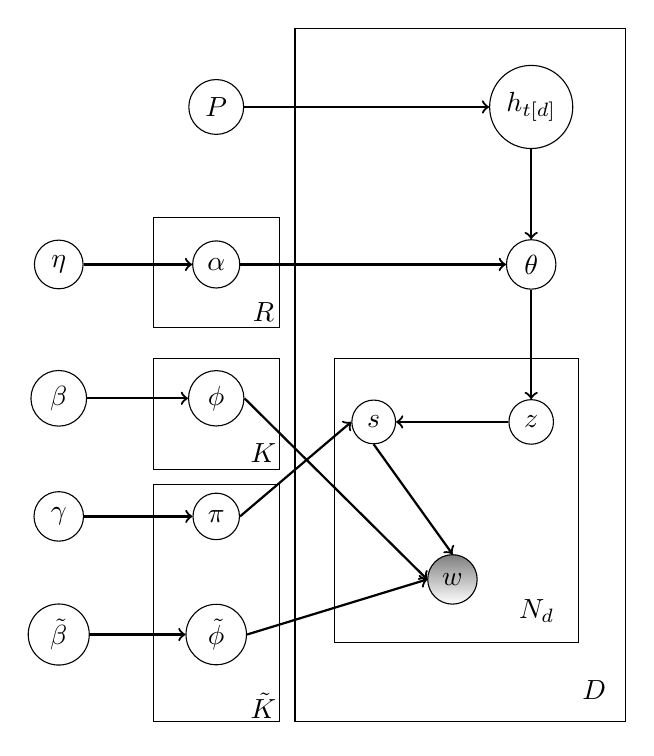
\begin{tikzpicture}
		\node (p) at (-4,2) [circle,draw] {$\bm{P}$};
		\node (htd) at (0,2) [circle,draw] {$h_{t[d]}$};
		\node (theta) at (0,0) [circle, draw] {$\theta$};
		\node (z) at (0,-2) [circle, draw] {$z$};
		\node (s) at (-2,-2) [circle, draw] {$s$};
		\node (a) at (-4,0) [circle, draw] {$\alpha$};
		\node (phi) at (-4,-1.7) [circle,draw] {$\phi$};
		\node (w) at (-1,-4) [shade,circle,draw] {$w$};
		\node (eta) at (-6,0) [circle,draw] {$\eta$};
		\node (beta) at (-6,-1.7) [circle,draw] {$\beta$};
		
		\node (gamma) at (-6,-3.2) [circle,draw] {$\gamma$};
		\node (pi) at (-4,-3.2) [circle,draw] {$\pi$};
		
		\node (tbeta) at (-6,-4.7) [circle,draw] {$\tilde{\beta}$};
		\node (tphi) at (-4,-4.7) [circle,draw] {$\tilde{\phi}$};
		
		
		\draw[thick,->] (p.east) -- (htd.west);
		\draw[thick,->] (a.east) -- (theta.west);
		\draw[thick,->] (phi.east) -- (w.west);
		\draw[thick,->] (z.west) -- (s.east);
		\draw[thick,->] (s.south) -- (w.north);
		\draw[thick,->] (eta.east) -- (a.west);
		\draw[thick,->] (beta.east) -- (phi.west);
		\draw[thick,->] (htd.south) -- (theta.north);
		\draw[thick,->] (theta.south) -- (z.north);
		
		\draw[thick,->] (gamma.east) -- (pi.west);
		\draw[thick,->] (tbeta.east) -- (tphi.west);
		
		\draw[thick,->] (pi.east) -- (s.west);
		\draw[thick,->] (tphi.east) -- (w.west);
		
		\draw (-3,-5.8) rectangle (1.2,3);
		\draw (-2.5,-4.8) rectangle (0.6,-1.2);
		\draw (-4.8,-0.8) rectangle (-3.2,0.6);
		
		\draw (-4.8,-2.6) rectangle (-3.2,-1.2);
		\draw (-4.8,-5.8) rectangle (-3.2,-2.8);
		
		\node at (0.07,-4.4) {$N_d$};
		
		\node at (0.8,-5.4) {$D$};
		
		\node at (-3.4,-0.6) {$R$};
		\node at (-3.4,-2.4) {$K$};	
		\node at (-3.4,-5.6) {$\tilde{K}$};
		
	\end{tikzpicture}
	\caption{Graphical model of dynamic \textsf{\textbf{keyATM}}}
	\label{graph:dynamickeyatm}
	\floatfoot{The shaded node ($w$) denotes observed variables, while other transparent nodes denote latent variables. Source: \cite[41]{Eshima.2020}}
\end{figure}	


%Modelfit Graphic
\begin{figure}[H]
	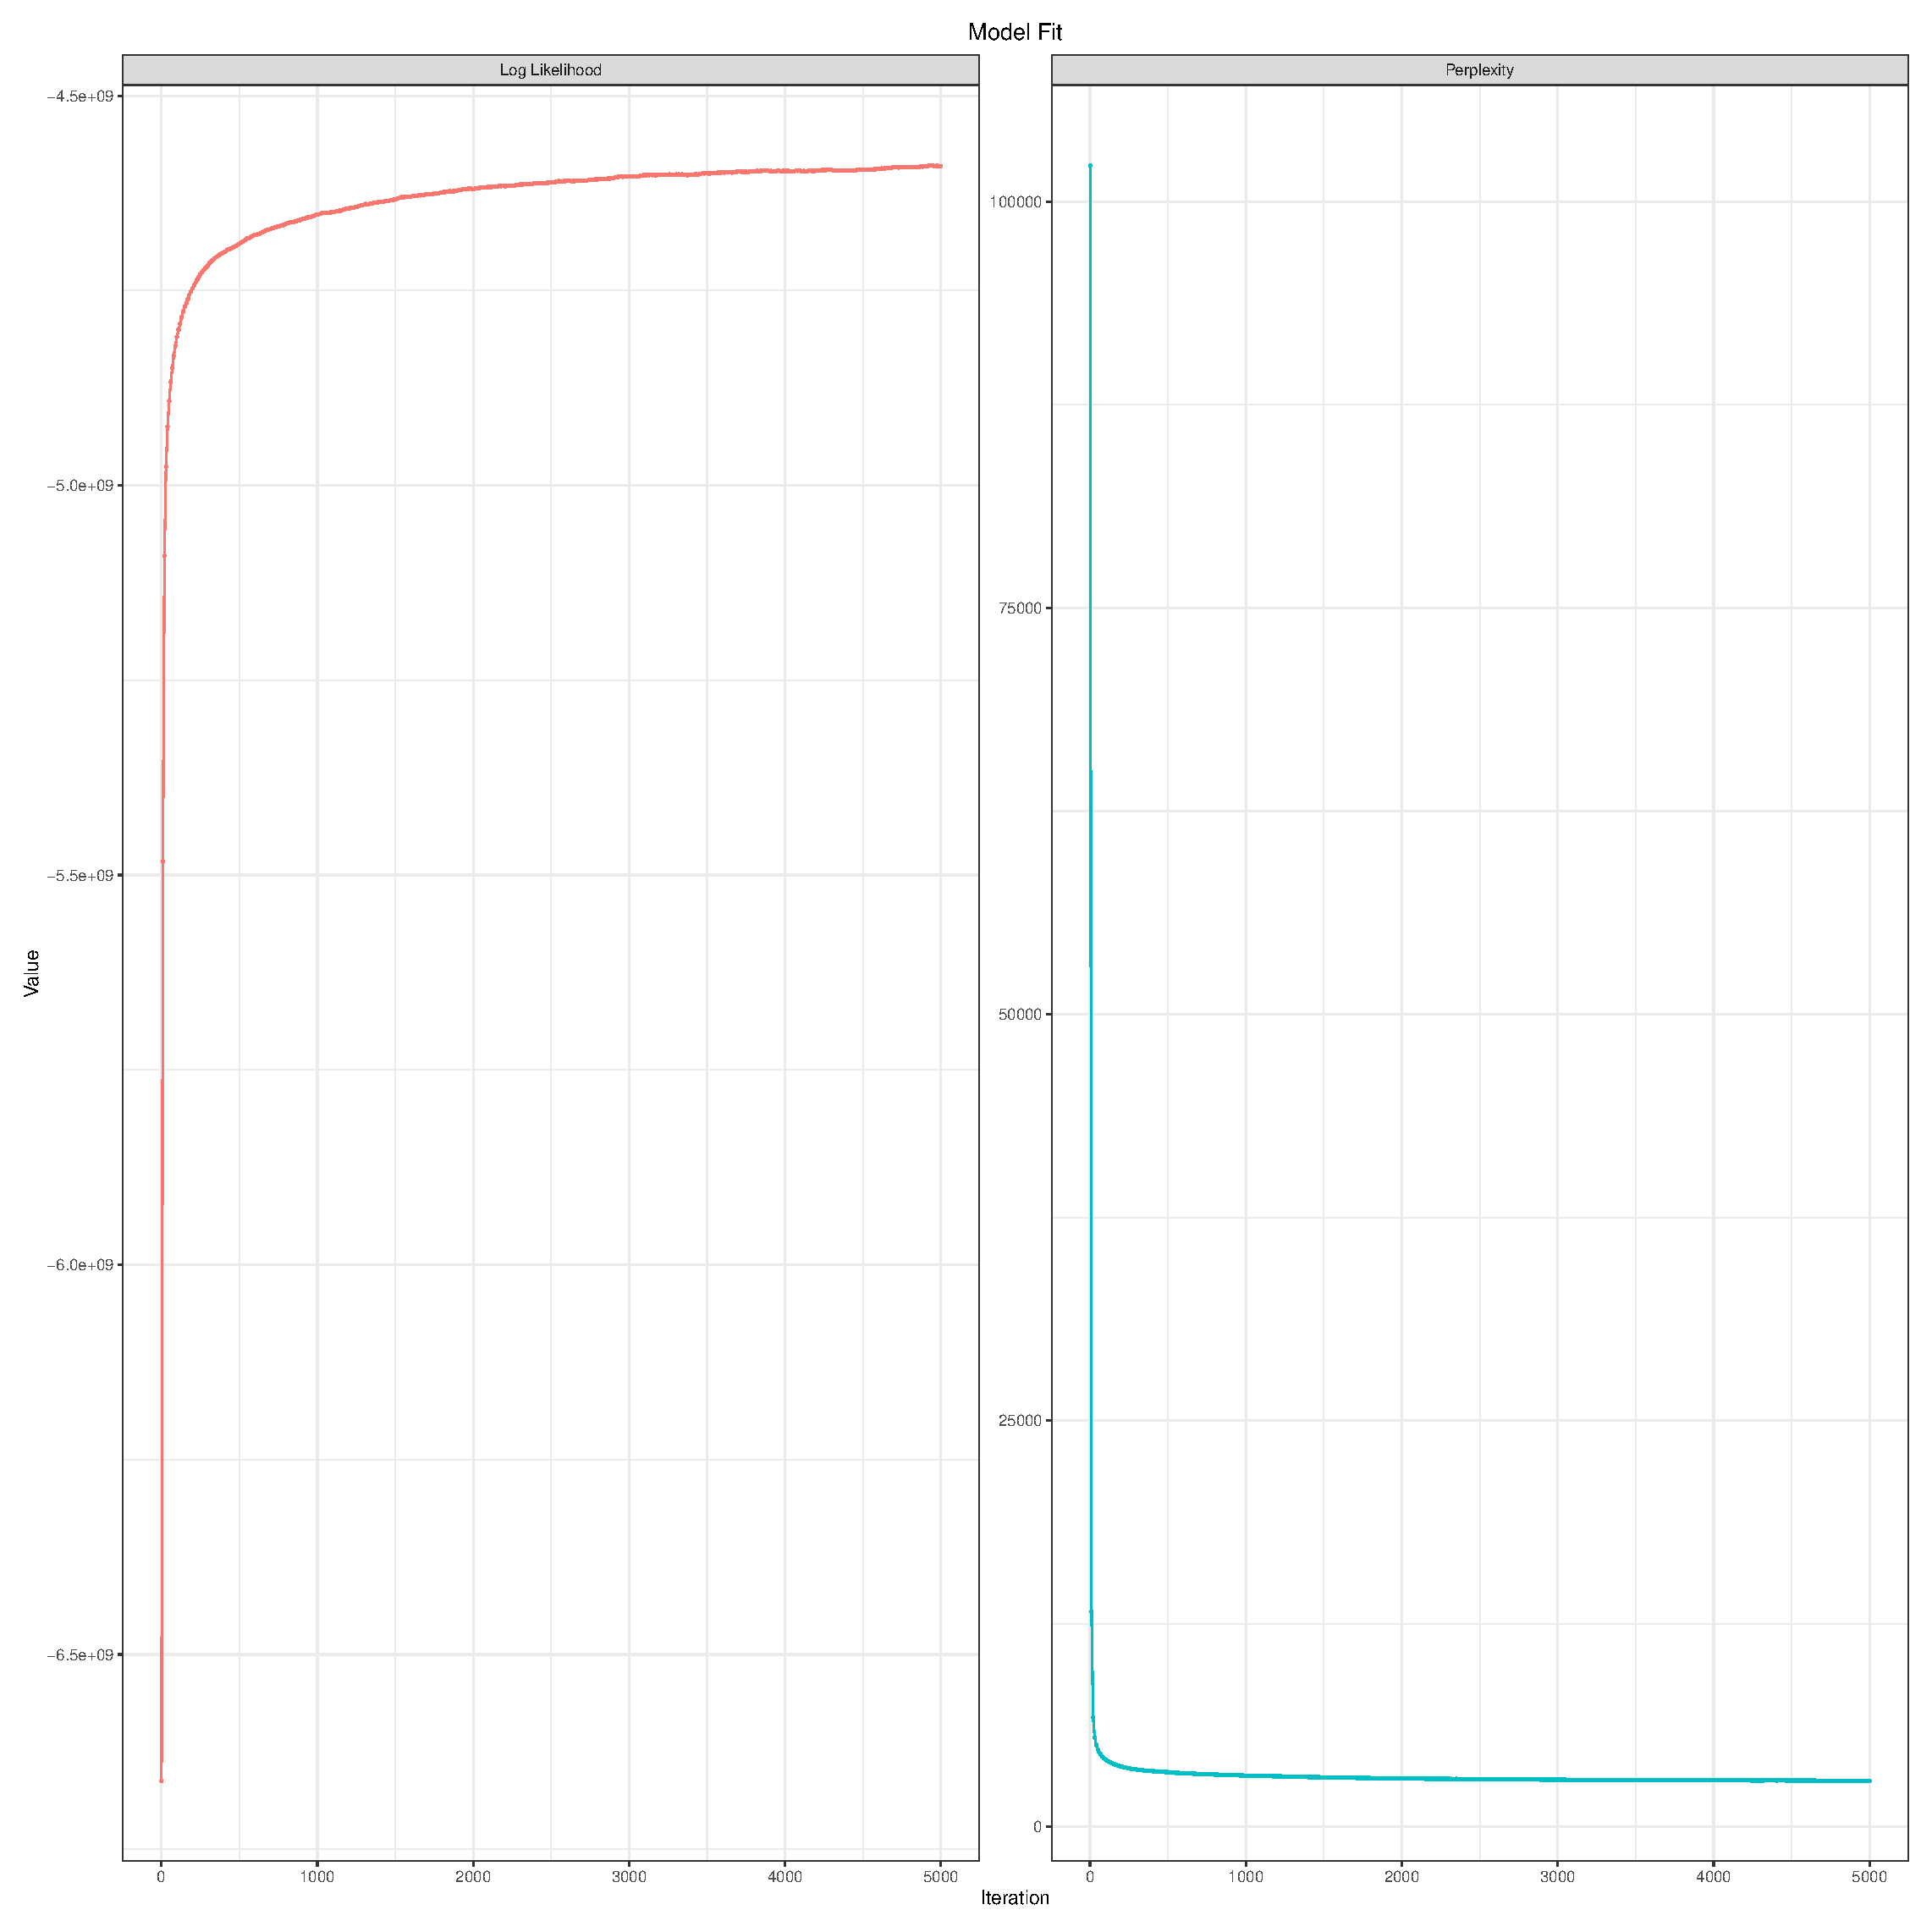
\includegraphics[width=1\linewidth]{figures/modelfit_djn_model.eps}
	\caption{Modelfit}
	\label{fig:modelfit}
\end{figure}

%Estimated Alpha
 \begin{figure}[H]
	\begin{center}
		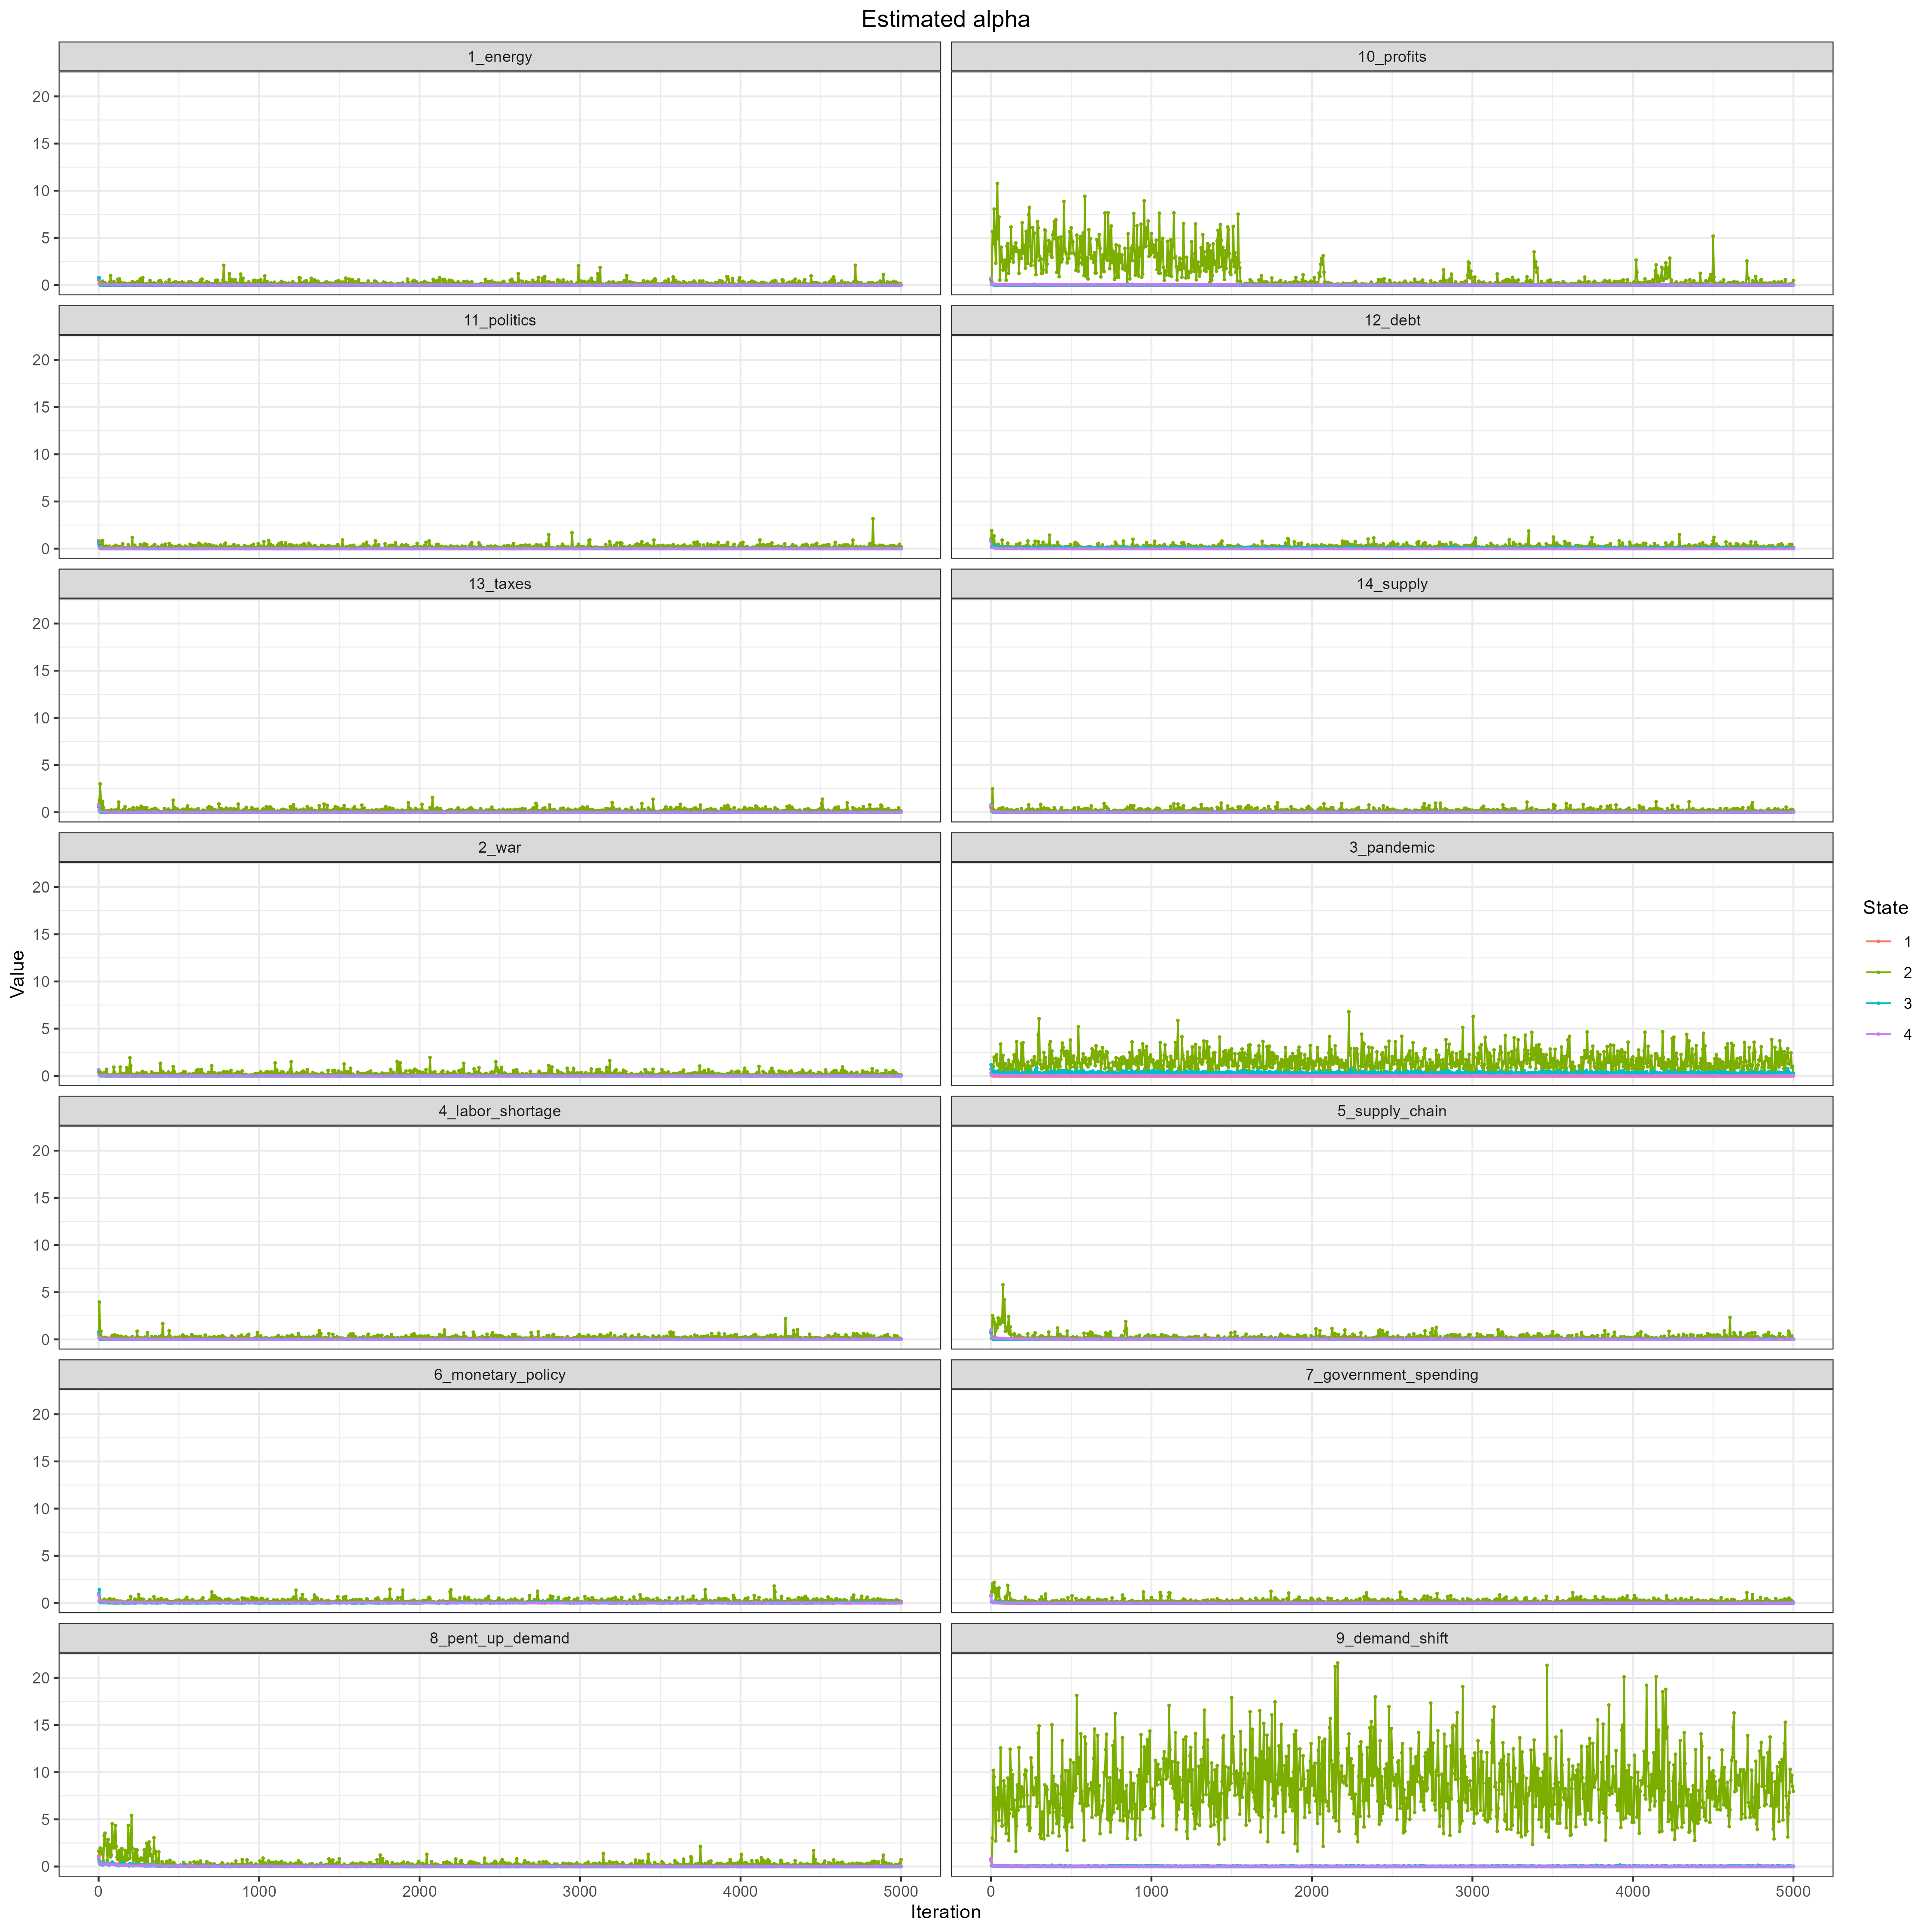
\includegraphics[width=1.0\linewidth]{figures/alpha_djn_model.eps}
		\caption{Estimated alpha}
		\label{fig:alpha}
	\end{center}
\end{figure}

%Top-20 Words

 %% latex table generated in R 4.2.3 by xtable 1.8-4 package
% Wed Aug 23 21:41:09 2023

\begin{sidewaystable}[H]
	\centering
	\footnotesize
	\begin{tabular}{p{0.3cm}|p{1.4cm}|p{1.4cm}|p{1.4cm}|p{1.4cm}|p{1.4cm}|p{1.4cm}|p{1.4cm}|p{1.4cm}|p{1.4cm}|p{1.4cm}|p{1.4cm}|p{1.4cm}|p{1.4cm}}
	\caption{Top-20 words per keyword topic}\label{table:top_words}
	& energy & war & pandemic & labor shortage & supply chain & monetary policy & government spending & pent-up demand & demand-shift & profits & politics & debt & taxes \\ 
	\hline
	1 & price & russia [\checkmark] & coronavirus & job [\checkmark] & company & fed [\checkmark] & u.s & growth & price & share & president [\checkmark] & bank & tax [\checkmark] \\ 
	2 & oil [\checkmark] & ukraine [\checkmark] & pandemic [\checkmark] & labor [\checkmark] & price & rate & china & economist & inflation & company & biden [\checkmark] & debt [\checkmark] & plan \\ 
	3 & high & russian & covid-19 [\checkmark] & worker [\checkmark] & supply [\checkmark] & inflation & trade & expect & consumer [\checkmark] & profit [\checkmark] & house & bond & cost \\ 
	4 & market & u.s & u.s & wage [\checkmark] & cost & bank & tariff & inflation & rise & market & election & rate & pay \\ 
	5 & us & oil [1] & recovery [8] & rate & new & policy & bank & rise & increase & expect & trump [\checkmark] & market & income \\ 
	6 & gas [\checkmark] & price & new & unemployment & chain [\checkmark] & powell & economy & economy & high & group & democrats [\checkmark] & government [\checkmark] & increase \\ 
	7 & week & energy & vaccine & economy & sale & central & trump [11] & economic & sale & revenue & party [\checkmark] & central & make \\ 
	8 & barrel & gas [1] & economic & work & vehicle [9] & interest & stock & quarter & quarter & rise & senate [\checkmark] & currency & billion \\ 
	9 & energy & war [\checkmark] & case [\checkmark] & growth & demand [8] & federal [12] & market & eurozone & rate & million & state & dollar & new \\ 
	10 & demand [8] & country & economy & high & car & market & chinese & price & spending [7] & price & vote & billion & energy \\ 
	11 & rise & sanction & variant & market & high & economy & rate & high & food & plc & government [\checkmark] & interest & bill \\ 
	12 & crude [\checkmark] & europe & week & u.s & business & official & growth & fall & early & quarter & administration [7] & investor & climate \\ 
	13 & future & supply [5] & stimulus [7] & people & maker & reserve & global & datum & u.s & growth & u.s & economy & price \\ 
	14 & production & invasion [\checkmark] & omicron & last & increase & raise [13] & price & sector & index & high & republicans & country & government [7] \\ 
	15 & low & european & restriction & low & make & increase & rise & activity & cost & sale & support & u.s & change \\ 
	16 & day & global & government [7] & economist & industry & point & economic & index & last & penny & political & financial & include \\ 
	17 & fall & official & china & time & last & meeting & president [11] & bank & economist & analyst & new & high & use \\ 
	18 & supply [5] & world & lockdown [8] & rise & executive & economic & new & remain & expect & first & white & yield & state \\ 
	19 & expect & high & country & inflation & u.s & expect & inflation & survey & good & u.k & former & economic & benefit \\ 
	20 & analyst & government [7] & demand [8] & pay & production & high & investor & gdp & fall & fall & leader & fund & high \\ 
		\hline
	
	\end{tabular}
\end{sidewaystable}



%Change in Mean

\begin{figure}[H]
	\centering
	\includegraphics[width=0.7\linewidth, angle = 270]{figures/plot_change.eps}
	\caption{Change of mean proportions}
	\label{fig:change}
	\floatfoot{Note: The Figure shows the change in mean proportions since 2021 with the 95\% confidence intervals. To calculate the relative proportions only the topics with pre-specified keywords were considered, so that the sum of the proportions of all keyword topics equals 1. All other non-keyword topics were excluded. We organized the topics by following the code system provided by \cite{Andre.2023}.}
\end{figure}




\begin{sidewaysfigure}[H]
	\centering
	\includegraphics[width=0.7\linewidth, angle = 270]{figures/comparision.eps}
	\caption{Change of mean proportions}
	\label{fig:comparision}
\end{sidewaysfigure}

\begin{sidewaystable}[H]
\centering
\caption{Elliott, Rothenberg and Stock unit root test results}\label{table:ers}

\begin{tabular}{lcccc}
\toprule
\textbf{Variable} & \textbf{Statistic} & \textbf{Critical Value 1\%} & \textbf{Critical Value 5\%} & \textbf{Critical Value 10\%} \\
\midrule
Government Spending & 1.6 & 1.95 & 3.11 & 4.17 \\
Monetary Policy & 5.22 & 1.95 & 3.11 & 4.17 \\
Demand & 3.73 & 1.95 & 3.11 & 4.17 \\
Demand Shift & 5.3 & 1.95 & 3.11 & 4.17 \\
Supply Chain & 4.3 & 1.95 & 3.11 & 4.17 \\
Energy & 2.17 & 1.95 & 3.11 & 4.17 \\
Labor Shortage & 9.01 & 1.95 & 3.11 & 4.17 \\
Supply & 3.44 & 1.95 & 3.11 & 4.17 \\
Pandemic & 2.03 & 1.95 & 3.11 & 4.17 \\
Politics & 4.85 & 1.95 & 3.11 & 4.17 \\
War & 0.83 & 1.95 & 3.11 & 4.17 \\
Debt & 4.72 & 1.95 & 3.11 & 4.17 \\
Taxes & 3.09 & 1.95 & 3.11 & 4.17 \\
Profits & 6.34 & 1.95 & 3.11 & 4.17 \\
\bottomrule
\end{tabular}
\end{sidewaystable}



\newpage


%robustness Granger

\begin{table}[ht]
\centering
\caption{Narrative $\rightarrow$ Expectations Granger causality (level)}\label{tab:granger_level}

\begin{tabular}{lcc}
\toprule
\textbf{Narratives} & \textbf{One-Year Expectations} & \textbf{Three-Year Expectations} \\
& (Pr($>$F)) & (Pr($>$F)) \\
\midrule
\multicolumn{3}{l}{\textbf{Demand}} \\
\midrule
Government Spending & 0.23 & 0.38 \\
Monetary Policy & 0.68 & 0.01 ** \\
Demand Shift & 0.02 ** & $<$0.01 *** \\
Demand (residual) & 0.31 & 0.13 \\
\midrule
\multicolumn{3}{l}{\textbf{Supply}} \\
\midrule
Supply Chain & $<$0.01 *** & 0.03 ** \\
Energy & 0.83 & 0.26 \\
Labor Shortage & 0.15 & 0.12 \\
Supply (residual) & 0.18 & $<$0.01 *** \\
\midrule
\multicolumn{3}{l}{\textbf{Miscellaneous}} \\
\midrule
Pandemic & 0.76 & 0.94 \\
Politics & 0.15 & 0.10 * \\
War & 0.76 & 0.24 \\
Debt & 0.79 & 0.07 * \\
Taxes & 0.56 & 0.50 \\
Profits & $<$0.01 *** & $<$0.01 *** \\
\midrule
\bottomrule
\textit{Note:}  & \multicolumn{2}{r}{$^{*}$p$<$0.1; $^{**}$p$<$0.05; $^{***}$p$<$0.01} \\
\bottomrule
\end{tabular}
\end{table}

\newpage
\begin{table}[ht]
\centering
\caption{Granger causality analysis (differences)}\label{table:granger}

\begin{tabular}{lcc}
\toprule
\textbf{Narratives} & \textbf{One-Year Expectations} & \textbf{Three-Year Expectations} \\
& (Pr($>$F)) & (Pr($>$F)) \\
\midrule
\multicolumn{3}{l}{\textbf{Demand}} \\
\midrule
Government Spending & 0.01 ** & 0.15 \\
Monetary Policy & 0.68 & 0.26 \\
Pent-up Demand & 0.91 & 0.86 \\
Demand Shift & $<$0.01 *** & 0.12 \\
\midrule
\multicolumn{3}{l}{\textbf{Supply}} \\
\midrule
Supply Chain & 0.02 ** & 0.08 * \\
Energy & 0.96 & 0.27 \\
Labor Shortage & 0.12 & 0.94 \\
\midrule
\multicolumn{3}{l}{\textbf{Miscellaneous}} \\
\midrule
Pandemic & 0.58 & 0.71 \\
Politics & 0.59 & 0.55 \\
War & 0.51 & 0.12 \\
Debt & 0.07 * & 0.97 \\
Taxes & 0.86 & 0.73 \\
Profits & 0.22 & 0.55 \\
\midrule
\bottomrule
\textit{Note:}  & \multicolumn{2}{r}{$^{*}$p$<$0.1; $^{**}$p$<$0.05; $^{***}$p$<$0.01} \\
\bottomrule
\end{tabular}
\end{table}

\newpage


% heterogeneity

\begin{sidewaystable}[ht]
\centering
\caption{Income: Granger causality analysis (bHP-Filter)}\label{table:granger}

\begin{tabular}{lcccccc}
 \toprule
\textbf{Narratives} & \textbf{1-Year Low Income} & \textbf{3-Year Low Income} & \textbf{1-Year Mid Income} & \textbf{3-Year Mid Income} & \textbf{1-Year High Income} & \textbf{3-Year High Income} \\
\midrule
\multicolumn{7}{l}{\textbf{Demand}} \\
\midrule
Government Spending & 0.48 & 0.19 & 0.52 & 0.06 * & 0.73 & 0.28 \\
Monetary Policy & 0.50 & 0.63 & 0.44 & 0.15 & 0.10 * & 0.11 \\
Pent-up Demand & $<$0.01 *** & 0.25 & 0.13 & 0.15 & 0.05 * & 0.30 \\
Demand Shift & 0.33 & 0.18 & 0.50 & 0.74 & 0.59 & 0.49 \\
\midrule
\multicolumn{7}{l}{\textbf{Supply}} \\
\midrule
Supply Chain & $<$0.01 *** & 0.08 * & 0.02 ** & 0.32 & 0.01 ** & 0.08 * \\
Energy & 0.37 & 0.11 & 0.96 & 0.26 & 0.94 & 0.60 \\
Labor Shortage & 0.25 & 0.44 & 0.11 & 0.99 & 0.17 & 0.94 \\
\midrule
\multicolumn{7}{l}{\textbf{Miscellaneous}} \\
\midrule
Pandemic & 0.43 & 0.74 & 0.15 & 0.45 & 0.25 & 0.07 * \\
Politics & 0.85 & 0.81 & 0.57 & 0.33 & 0.88 & 0.56 \\
War & $<$0.01 *** & 0.10 * & 0.03 ** & 0.59 & 0.10 * & 0.25 \\
Debt & 0.36 & 0.74 & 0.35 & 0.95 & 0.27 & 0.36 \\
Taxes & 0.26 & 0.65 & 0.46 & 0.91 & 0.92 & 0.56 \\
Profits & $<$0.01 *** & 0.04 ** & 0.04 ** & 0.28 & 0.12 & $<$0.01 *** \\
\midrule
\bottomrule
\textit{Note:}  & \multicolumn{6}{r}{$^{*}$p$<$0.1; $^{**}$p$<$0.05; $^{***}$p$<$0.01} \\
\bottomrule
\end{tabular}
\end{sidewaystable}


\newpage

\begin{sidewaystable}[H]
\centering
\footnotesize
\caption{Education: Narrative $\rightarrow$ Expectations Granger causality (bHP-Filter)}\label{table:granger}

\begin{tabular}{lcccccc}
\toprule
\textbf{Narratives} & \textbf{1-Year Low Education} & \textbf{3-Year Low Education} & \textbf{1-Year Mid Education} & \textbf{3-Year Mid Education} & \textbf{1-Year High Education} & \textbf{3-Year High Education} \\
\midrule
\multicolumn{7}{l}{\textbf{Demand}} \\
\midrule
Government Spending & 0.01 ** & $<$0.01 *** & 0.74 & $<$0.01 *** & 0.37 & 0.08 * \\
Monetary Policy & 0.16 & 0.57 & 0.71 & 0.29 & 0.52 & 0.65 \\
Demand Shift & $<$0.01 *** & 0.63 & 0.48 & 0.77 & 0.01 ** & $<$0.01 *** \\
Demand (residual) & 0.22 & 0.29 & 0.72 & 0.45 & 0.49 & 0.87 \\
\midrule
\multicolumn{7}{l}{\textbf{Supply}} \\
\midrule
Supply Chain & $<$0.01 *** & 0.50 & 0.10 * & 0.08 * & $<$0.01 *** & 0.01 ** \\
Energy & 0.43 & 0.62 & 0.08 * & 0.06 * & 0.28 & 0.10 * \\
Labor Shortage & 0.10 * & 0.80 & 0.02 ** & 0.84 & 0.24 & 0.61 \\
Supply (residual) & 0.04 ** & 0.58 & 0.45 & 0.38 & 0.02 ** & 0.03 ** \\
\midrule
\multicolumn{7}{l}{\textbf{Miscellaneous}} \\
\midrule
Pandemic & 0.14 & 0.94 & 0.17 & 0.90 & 0.25 & 0.15 \\
Politics & 0.13 & 0.93 & 0.61 & 0.21 & 0.40 & 0.25 \\
War & $<$0.01 *** & 0.66 & $<$0.01 *** & 0.04 ** & 0.19 & 0.04 ** \\
Debt & 0.68 & 0.39 & 0.31 & 0.44 & 0.28 & 0.12 \\
Taxes & 0.28 & 0.71 & 0.75 & 0.53 & 0.94 & 0.87 \\
Profits & $<$0.01 *** & 0.14 & 0.08 * & 0.05 * & 0.02 ** & $<$0.01 *** \\
\midrule
\bottomrule
\textit{Note:}  & \multicolumn{6}{r}{$^{*}$p$<$0.1; $^{**}$p$<$0.05; $^{***}$p$<$0.01} \\
\bottomrule
\end{tabular}
\end{sidewaystable}


\newpage

\begin{sidewaystable}[H]
\centering
\footnotesize
\caption{Age: Narrative $\rightarrow$ Expectations Granger causality (bHP-Filter)}\label{table:granger}

\begin{tabular}{lcccccc}
\toprule
\textbf{Narratives} & \textbf{1-Year Low Age} & \textbf{3-Year Low Age} & \textbf{1-Year Mid Age} & \textbf{3-Year Mid Age} & \textbf{1-Year High Age} & \textbf{3-Year High Age} \\
\midrule
\multicolumn{7}{l}{\textbf{Demand}} \\
\midrule
Government Spending & 0.95 & 0.02 ** & 0.11 & $<$0.01 *** & 0.33 & 0.02 ** \\
Monetary Policy & 0.61 & 0.74 & 0.59 & 0.73 & 0.47 & 0.10 \\
Demand Shift & 0.17 & 0.11 & 0.14 & 0.07 * & 0.06 * & 0.92 \\
Demand (residual) & 0.34 & 0.56 & 0.25 & 0.93 & 0.75 & 0.10 \\
\midrule
\multicolumn{7}{l}{\textbf{Supply}} \\
\midrule
Supply Chain & 0.01 ** & 0.03 ** & $<$0.01 *** & $<$0.01 *** & 0.02 ** & 0.10 * \\
Energy & 0.94 & 0.07 * & 0.06 * & 0.41 & 0.82 & 0.16 \\
Labor Shortage & 0.54 & 0.80 & 0.09 * & 0.70 & 0.03 ** & 0.31 \\
Supply (residual) & 0.72 & 0.36 & 0.36 & 0.70 & 0.05 * & 0.24 \\
\midrule
\multicolumn{7}{l}{\textbf{Miscellaneous}} \\
\midrule
Pandemic & 0.14 & 0.14 & 0.84 & 0.26 & 0.28 & 0.72 \\
Politics & 0.59 & 0.50 & 0.24 & 0.61 & 0.25 & 0.59 \\
War & 0.01 ** & $<$0.01 *** & 0.10 * & 0.10 & 0.03 ** & 0.62 \\
Debt & 0.04 ** & 0.96 & 0.69 & 0.52 & 0.25 & 0.79 \\
Taxes & 0.93 & 0.36 & 0.78 & 0.30 & 0.48 & 0.49 \\
Profits & 0.02 ** & $<$0.01 *** & 0.02 ** & $<$0.01 *** & 0.03 ** & 0.03 ** \\
\midrule
\bottomrule
\textit{Note:}  & \multicolumn{6}{r}{$^{*}$p$<$0.1; $^{**}$p$<$0.05; $^{***}$p$<$0.01} \\
\bottomrule
\end{tabular}
\end{sidewaystable}


\newpage
\begin{sidewaystable}[H]
\centering
\footnotesize
\caption{Numeracy: Narrative $\rightarrow$ Expectations Granger causality (bHP-Filter)}\label{tab:granger_bHP_num}

\begin{tabular}{lcccc}
\toprule
\textbf{Narratives} & \textbf{1-Year Low Numeracy} & \textbf{3-Year Low Numeracy} & \textbf{1-Year High Numeracy} & \textbf{3-Year High Numeracy} \\
\midrule
\multicolumn{5}{l}{\textbf{Demand}} \\
\midrule
Government Spending & 0.51 & 0.07 * & 0.24 & 0.06 * \\
Monetary Policy & 0.39 & 0.40 & 0.39 & 0.46 \\
Demand Shift & 0.39 & 0.70 & 0.15 & 0.61 \\
Demand (residual) & 0.43 & 0.55 & 0.38 & 0.36 \\
\midrule
\multicolumn{5}{l}{\textbf{Supply}} \\
\midrule
Supply Chain & 0.01 ** & 0.53 & $<$0.01 *** & 0.54 \\
Energy & 0.36 & 0.15 & 0.84 & 0.14 \\
Labor Shortage & 0.07 * & 0.96 & $<$0.01 *** & 0.95 \\
Supply (residual) & 0.98 & 0.59 & 0.19 & 0.58 \\
\midrule
\multicolumn{5}{l}{\textbf{Miscellaneous}} \\
\midrule
Pandemic & 0.14 & 0.67 & 0.29 & 0.99 \\
Politics & 0.69 & 0.22 & 0.36 & 0.24 \\
War & $<$0.01 *** & 0.02 ** & 0.05 ** & 0.06 * \\
Debt & 0.25 & 0.19 & 0.11 & 0.15 \\
Taxes & 0.18 & 0.44 & 0.99 & 0.40 \\
Profits & 0.06 * & 0.04 ** & 0.03 ** & 0.04 ** \\
\midrule
\bottomrule
\textit{Note:}  & \multicolumn{4}{r}{$^{*}$p$<$0.1; $^{**}$p$<$0.05; $^{***}$p$<$0.01} \\
\bottomrule
\end{tabular}
\end{sidewaystable}




% Irfs complete

\newpage
\begin{sidewaysfigure}[H]
	\centering
	\captionsetup{font=footnotesize}
	\begin{subfigure}{00.24\textwidth}
		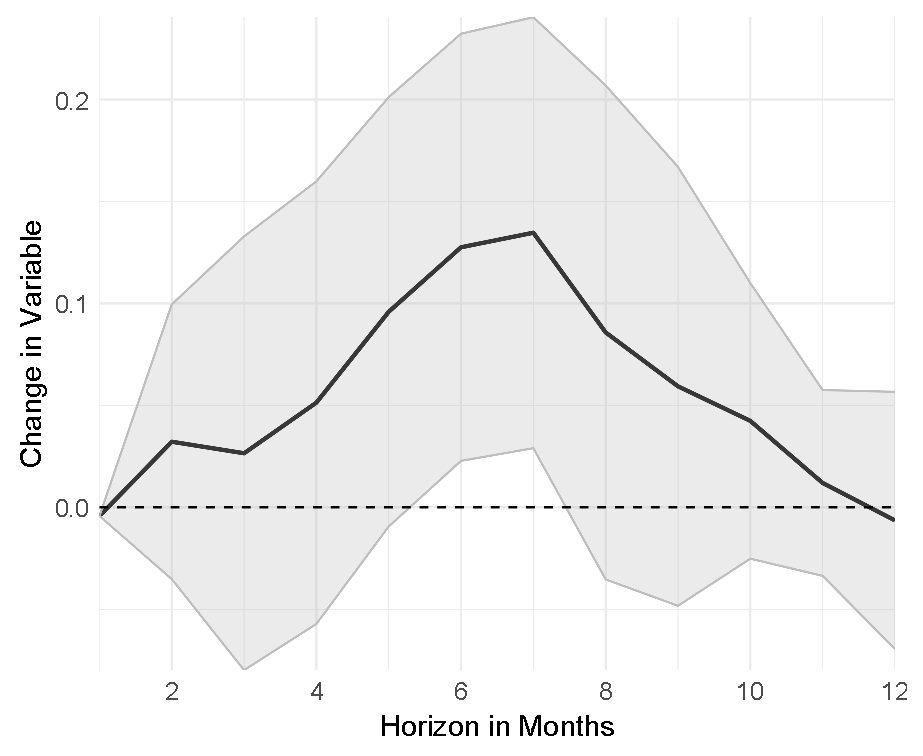
\includegraphics[width=0.8\textwidth]{output/lp/baseline/bHP/government_spending/government_spendingonexpectations1y_djn.eps}
		\caption{Government spending on 1-year expectations}
	\end{subfigure}
	\begin{subfigure}{00.24\textwidth}
		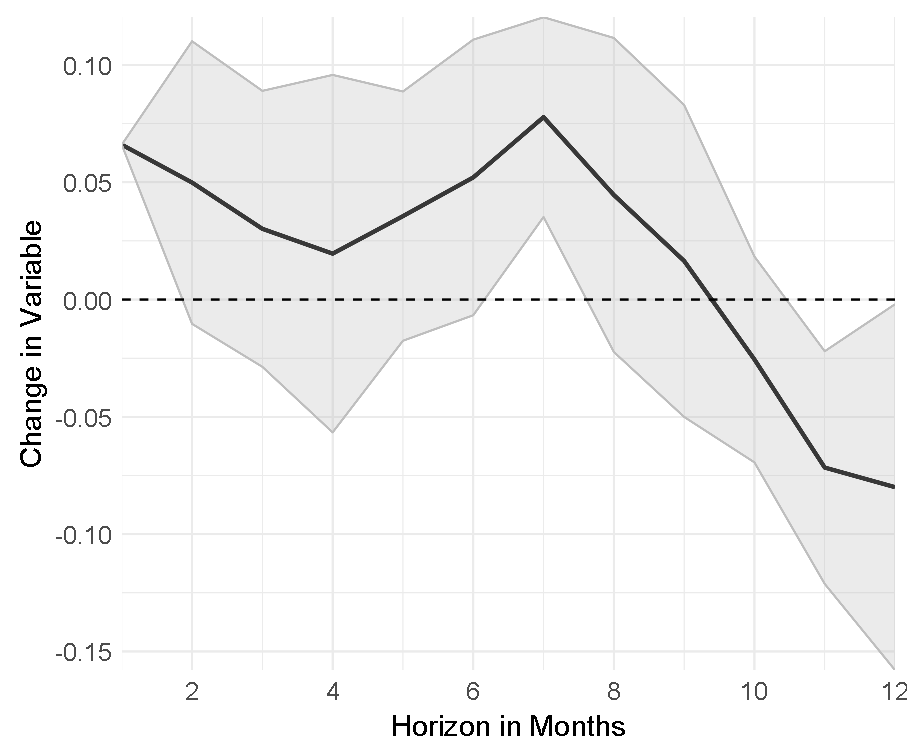
\includegraphics[width=0.8\textwidth]{output/lp/baseline/bHP/government_spending/government_spendingonexpectations3y_djn.eps}
		\caption{Government spending on 3-year expectations}
	\end{subfigure}
	\begin{subfigure}{00.24\textwidth}
	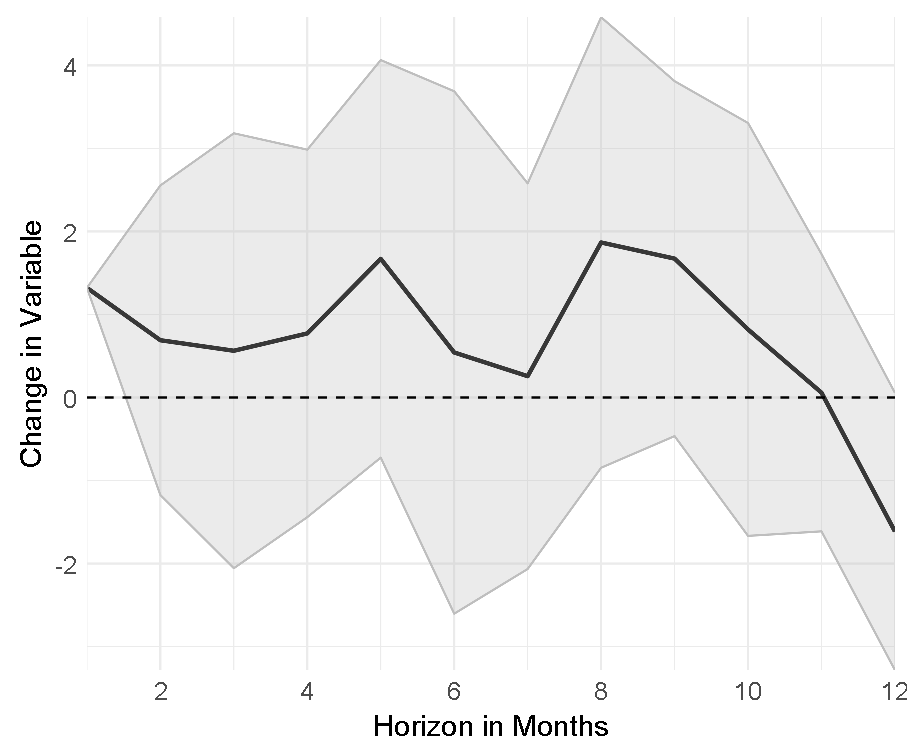
\includegraphics[width=0.8\textwidth]{output/lp/baseline/bHP/government_spending/government_spendingoninflation_djn.eps}
	\caption{Government spending on CPI inflation}
	\end{subfigure}
	\begin{subfigure}{00.24\textwidth}
		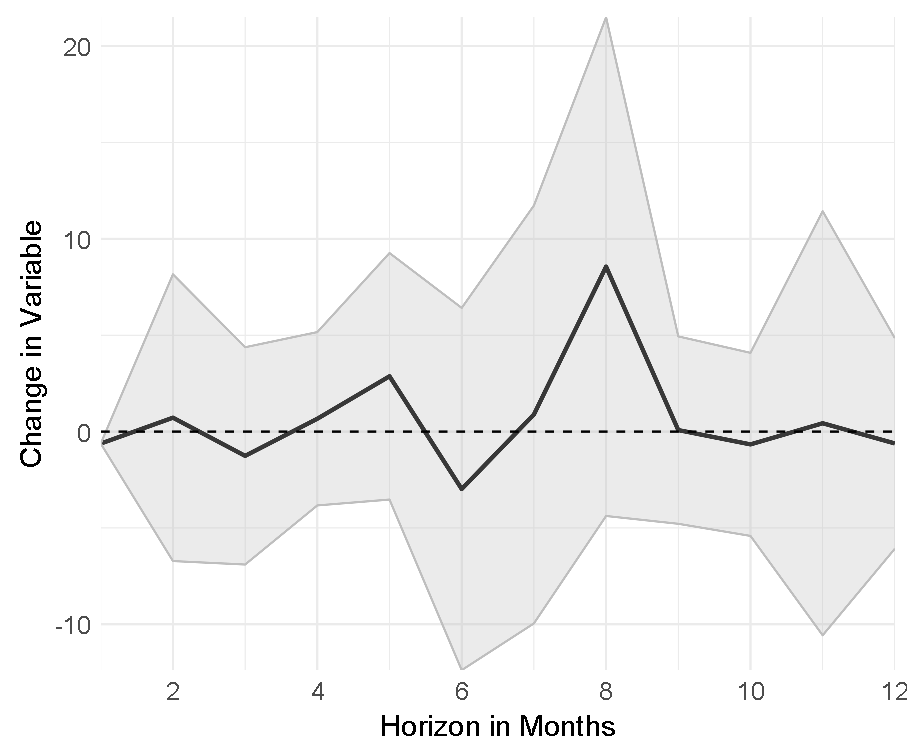
\includegraphics[width=0.8\textwidth]{output/lp/baseline/bHP/government_spending/government_spendingoneconac_djn.eps}
		\caption{Government spending on economic activity}
	\end{subfigure}
	\begin{subfigure}{00.24\textwidth}
		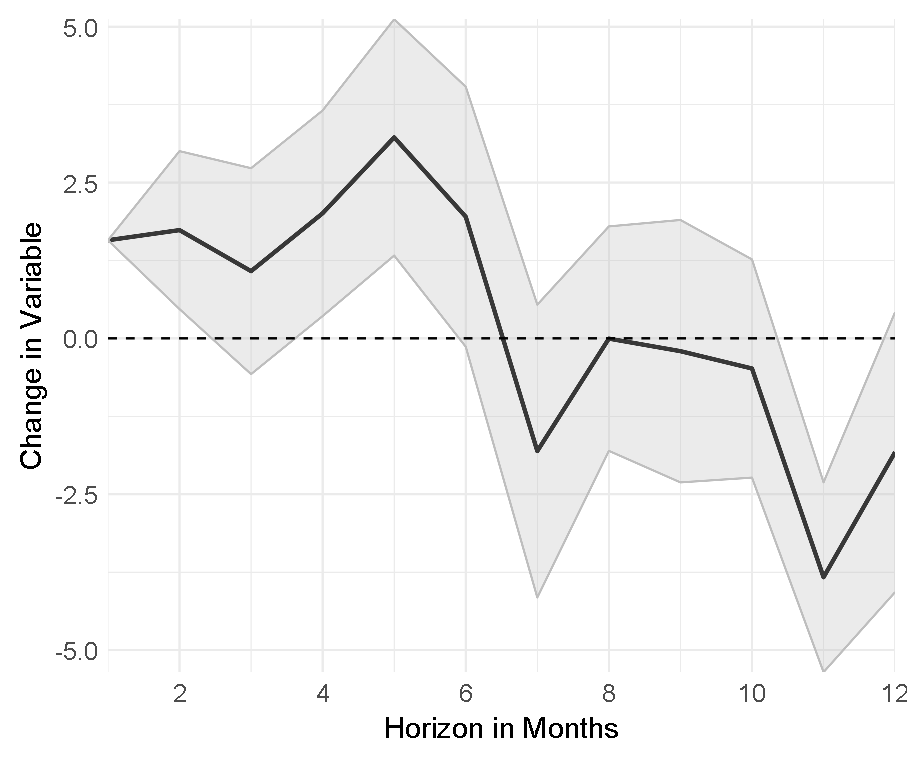
\includegraphics[width=0.8\textwidth]{output/lp/baseline/bHP/monetary_policy/monetary_policyonexpectations1y_djn.eps}
		\caption{Monetary policy on 1-year expectations}
	\end{subfigure}
	\begin{subfigure}{00.24\textwidth}
		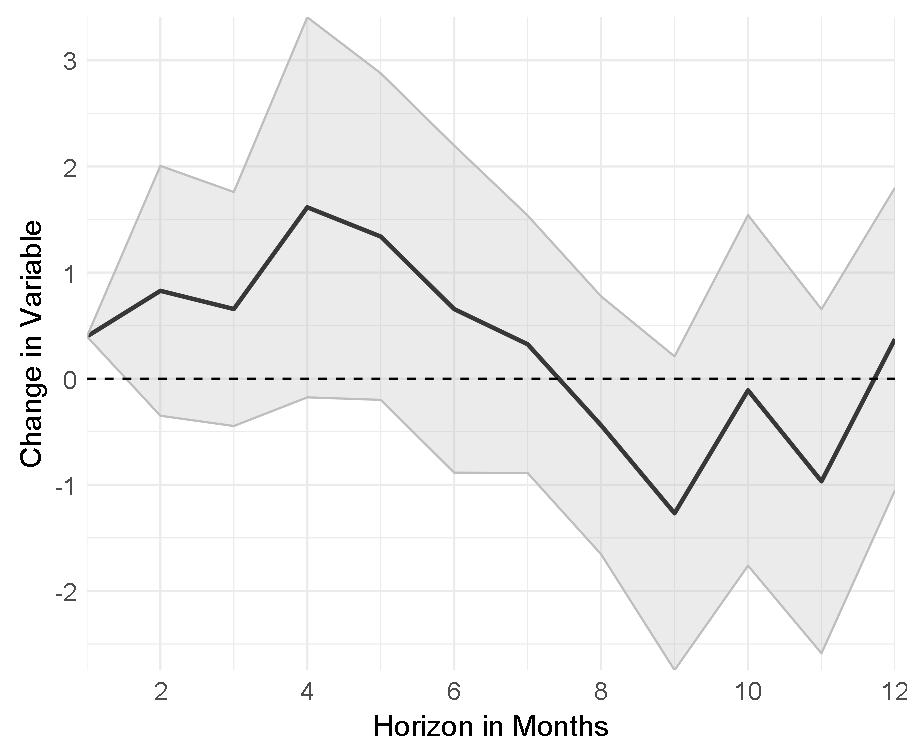
\includegraphics[width=0.8\textwidth]{output/lp/baseline/bHP/monetary_policy/monetary_policyonexpectations3y_djn.eps}
		\caption{Monetary policy on 3-year expectations}
	\end{subfigure}
	\begin{subfigure}{00.24\textwidth}
		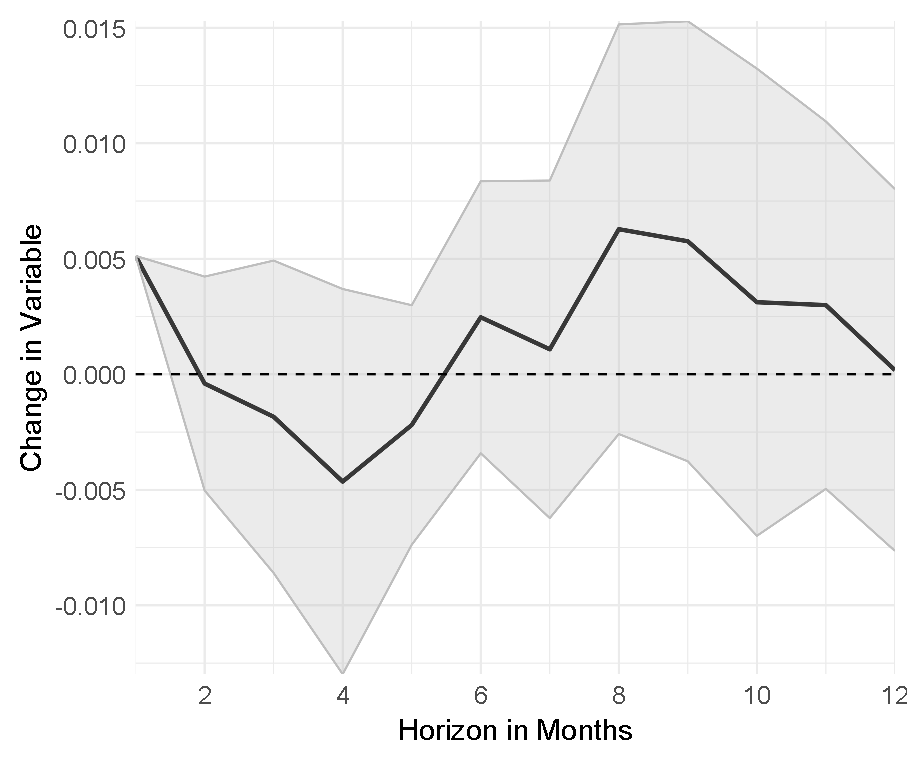
\includegraphics[width=0.8\textwidth]{output/lp/baseline/bHP/monetary_policy/monetary_policyoninflation_djn.eps}
		\caption{Monetary policy on CPI inflation}
	\end{subfigure}
	\begin{subfigure}{00.24\textwidth}
		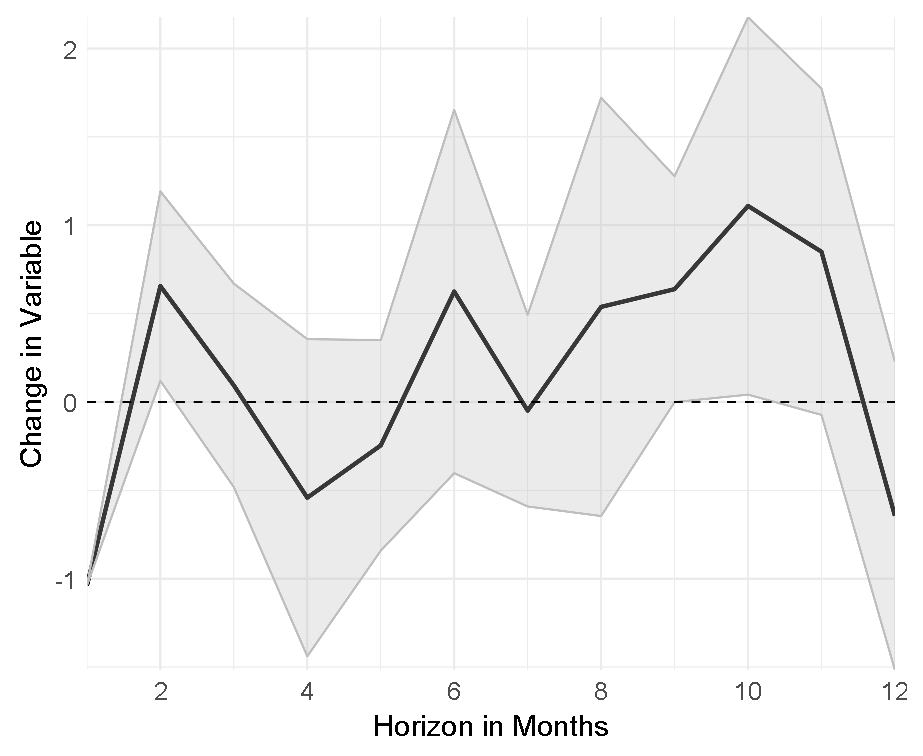
\includegraphics[width=0.8\textwidth]{output/lp/baseline/bHP/monetary_policy/monetary_policyoneconac_djn.eps}
		\caption{Monetary policy on economic activity}
	\end{subfigure}
	\begin{subfigure}{00.24\textwidth}
		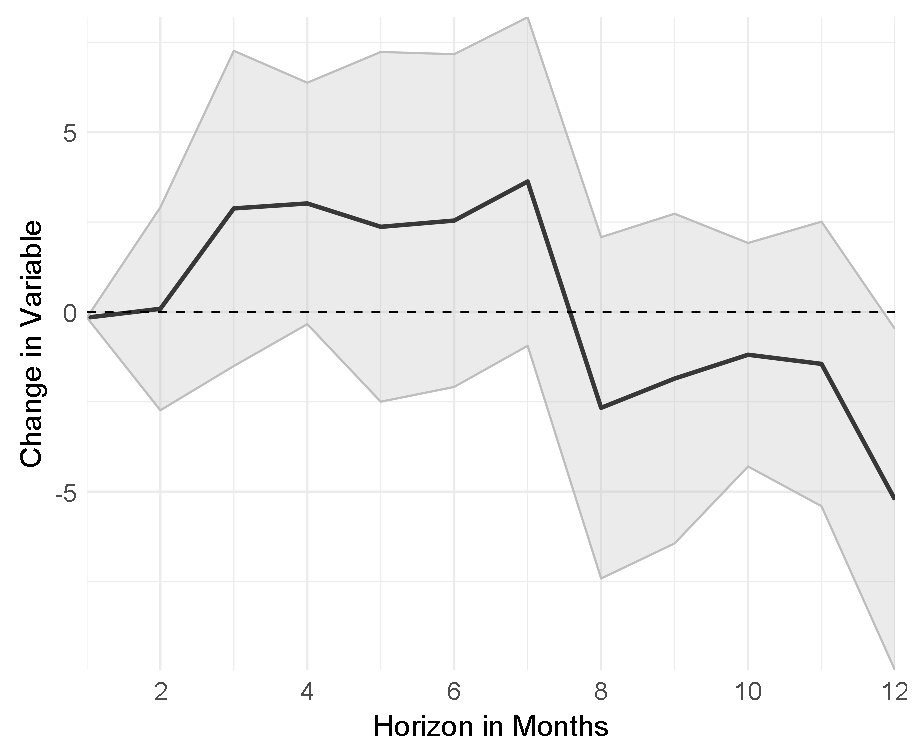
\includegraphics[width=0.8\textwidth]{output/lp/baseline/bHP/demand/demandonexpectations1y_djn.eps}
		\caption{Demand (residual) on 1-year expectations}
	\end{subfigure}
	\begin{subfigure}{00.24\textwidth}
		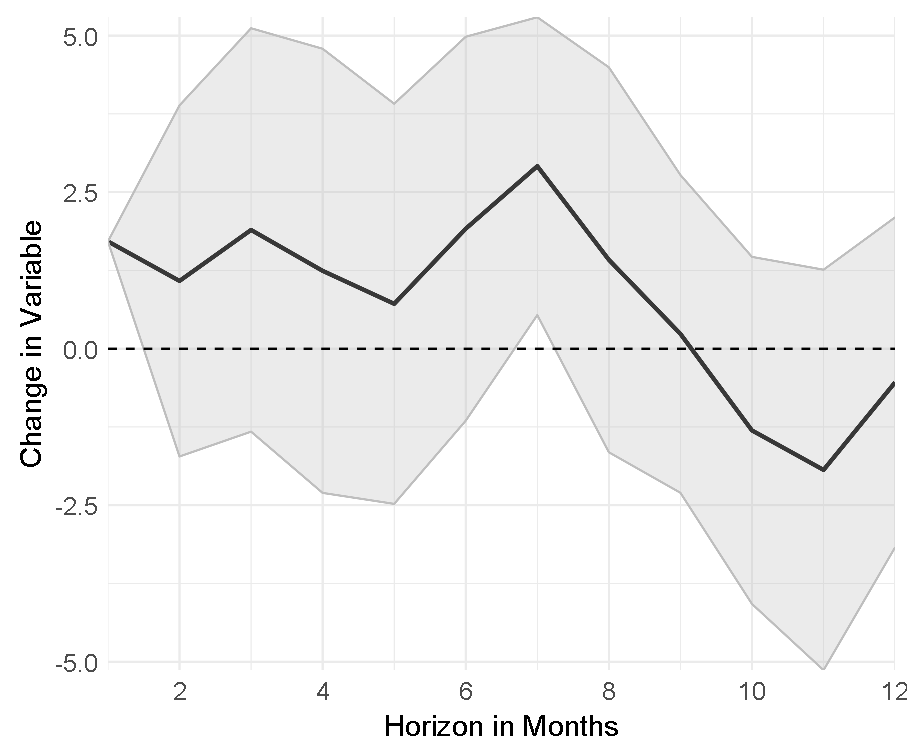
\includegraphics[width=0.8\textwidth]{output/lp/baseline/bHP/demand/demandonexpectations3y_djn.eps}
		\caption{Demand (residual) on 3-year expectations}
	\end{subfigure}
	\begin{subfigure}{00.24\textwidth}
		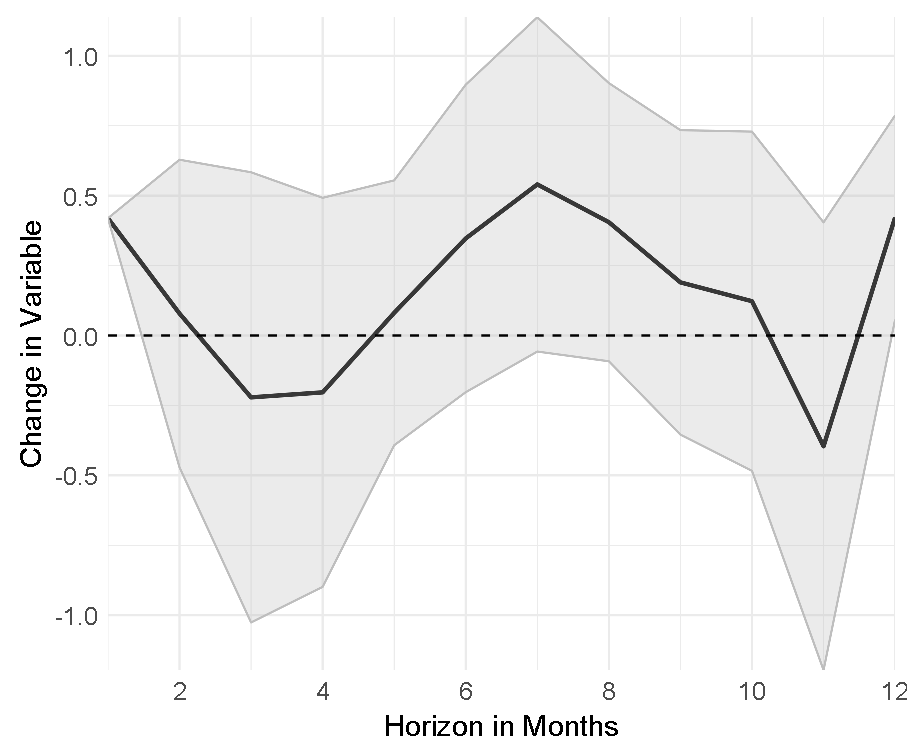
\includegraphics[width=0.8\textwidth]{output/lp/baseline/bHP/demand/demandoninflation_djn.eps}
		\caption{Demand (residual) on CPI inflation}
	\end{subfigure}
	\begin{subfigure}{00.24\textwidth}
		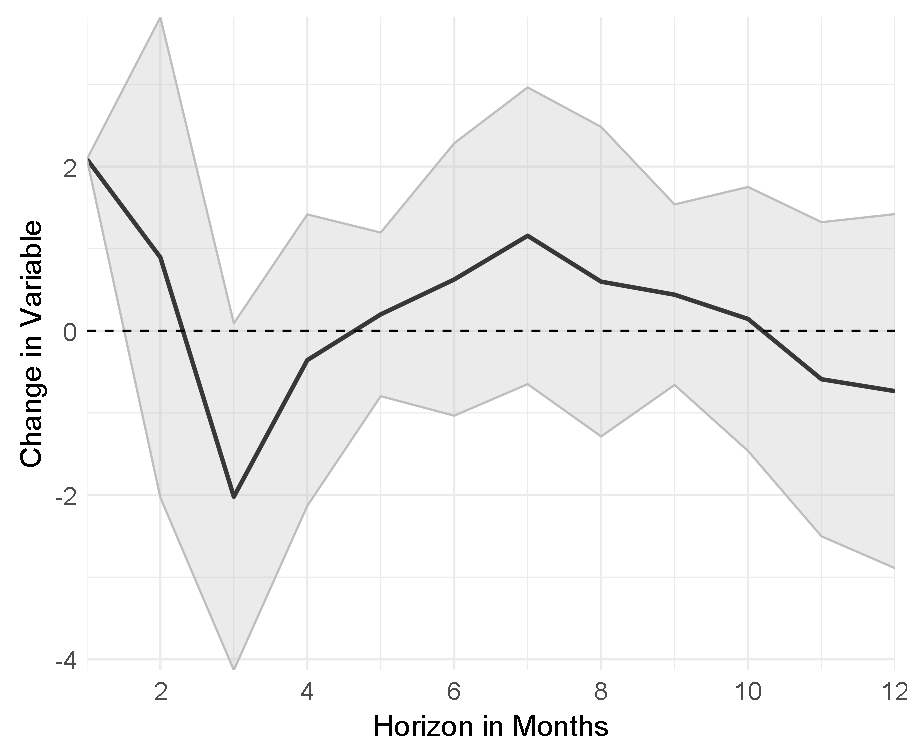
\includegraphics[width=0.8\textwidth]{output/lp/baseline/bHP/demand/demandoneconac_djn.eps}
		\caption{Demand (residual) on economic activity}
	\end{subfigure}
	\begin{subfigure}{00.24\textwidth}
		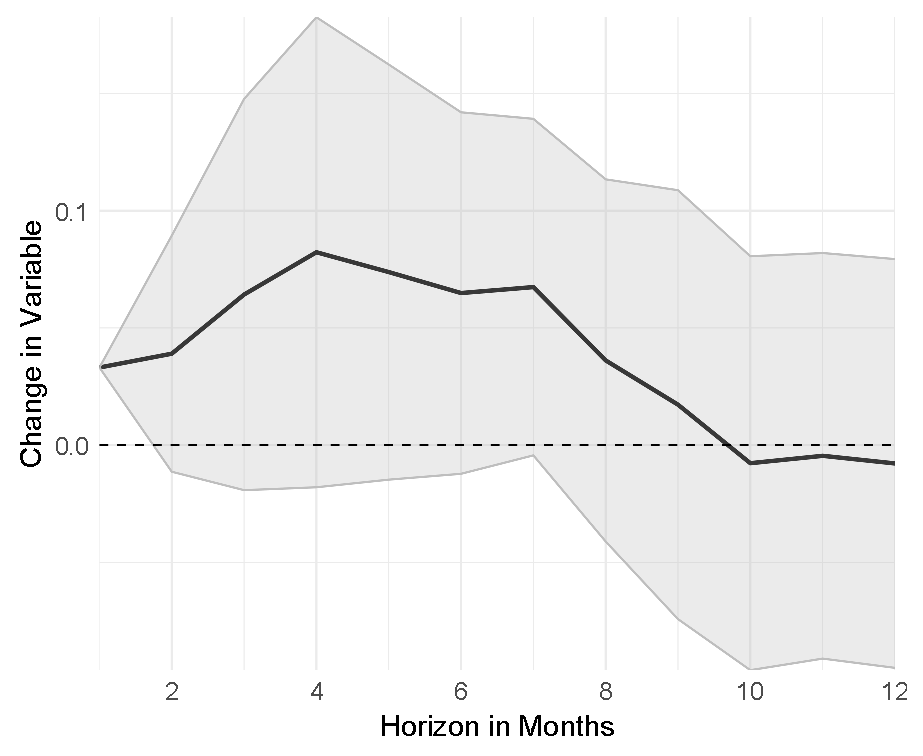
\includegraphics[width=0.8\textwidth]{output/lp/baseline/bHP/demand_shift/demand_shiftonexpectations1y_djn.eps}
		\caption{Demand shift on 1-year expectations}
	\end{subfigure}
	\begin{subfigure}{00.24\textwidth}
		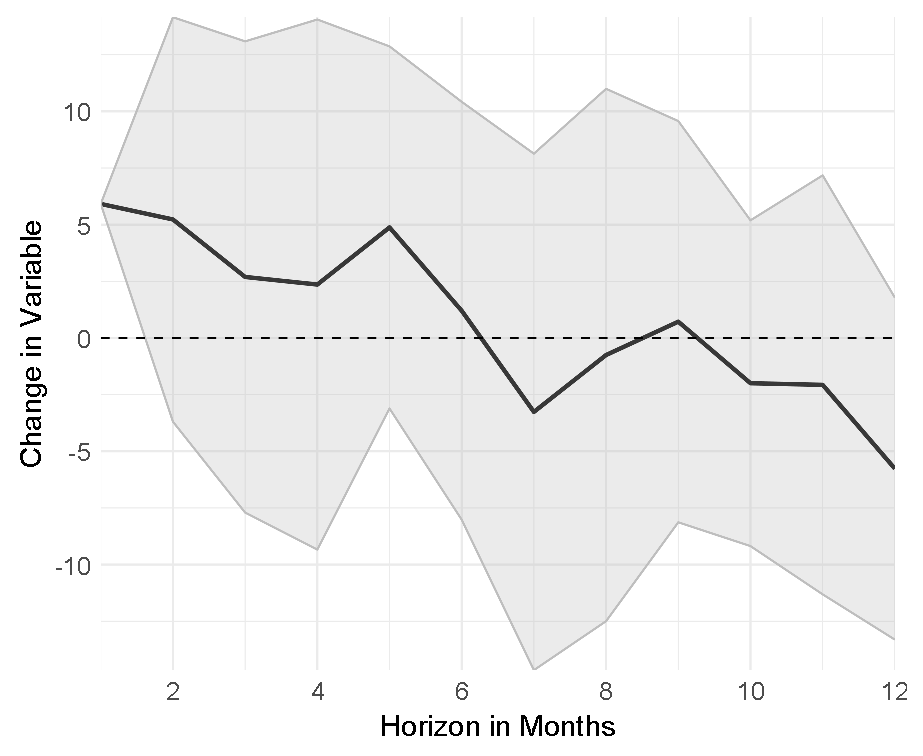
\includegraphics[width=0.8\textwidth]{output/lp/baseline/bHP/demand_shift/demand_shiftonexpectations3y_djn.eps}
		\caption{Demand shift on 3-year expectations}
	\end{subfigure}
	\begin{subfigure}{00.24\textwidth}
		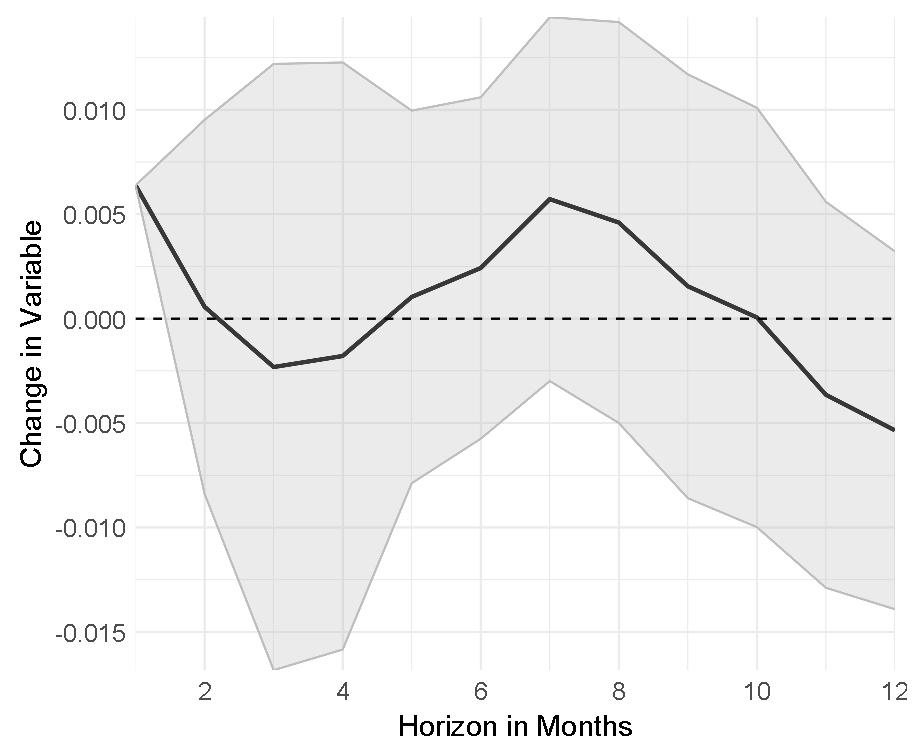
\includegraphics[width=0.8\textwidth]{output/lp/baseline/bHP/demand_shift/demand_shiftoninflation_djn.eps}
		\caption{Demand shift on CPI inflation}
	\end{subfigure}
	\begin{subfigure}{00.24\textwidth}
		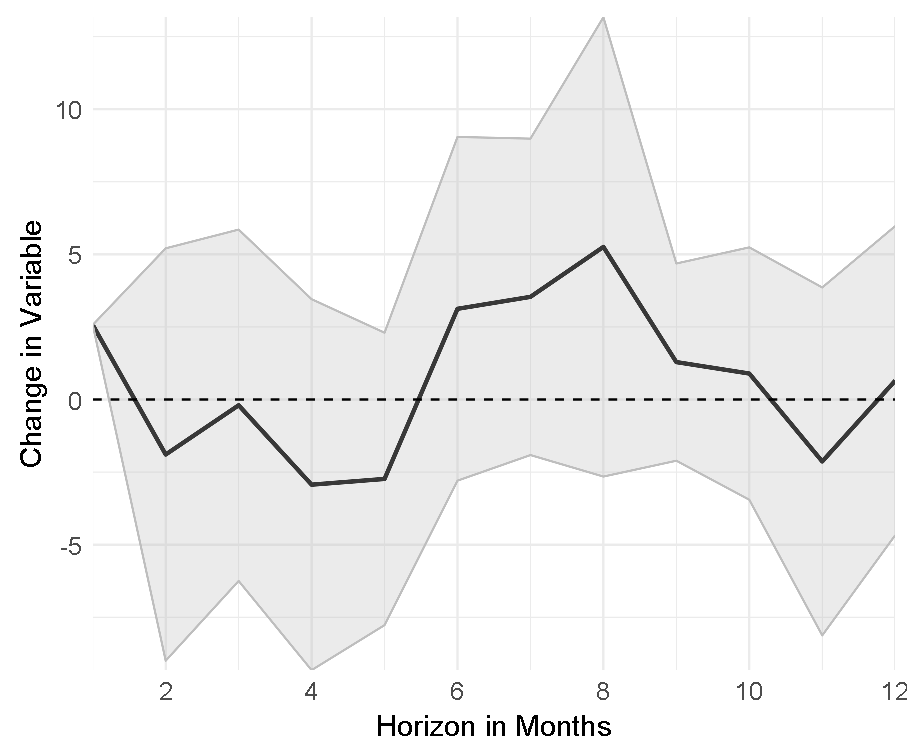
\includegraphics[width=0.8\textwidth]{output/lp/baseline/bHP/demand_shift/demand_shiftoneconac_djn.eps}
		\caption{Demand shift on economic activity}
	\end{subfigure}
	\caption{Demand narratives' impulse responses}
	\label{fig:irf_1}
\end{sidewaysfigure}

\newpage
\begin{sidewaysfigure}[H]
	\centering
	\captionsetup{font=footnotesize}
	\begin{subfigure}{00.24\textwidth}
		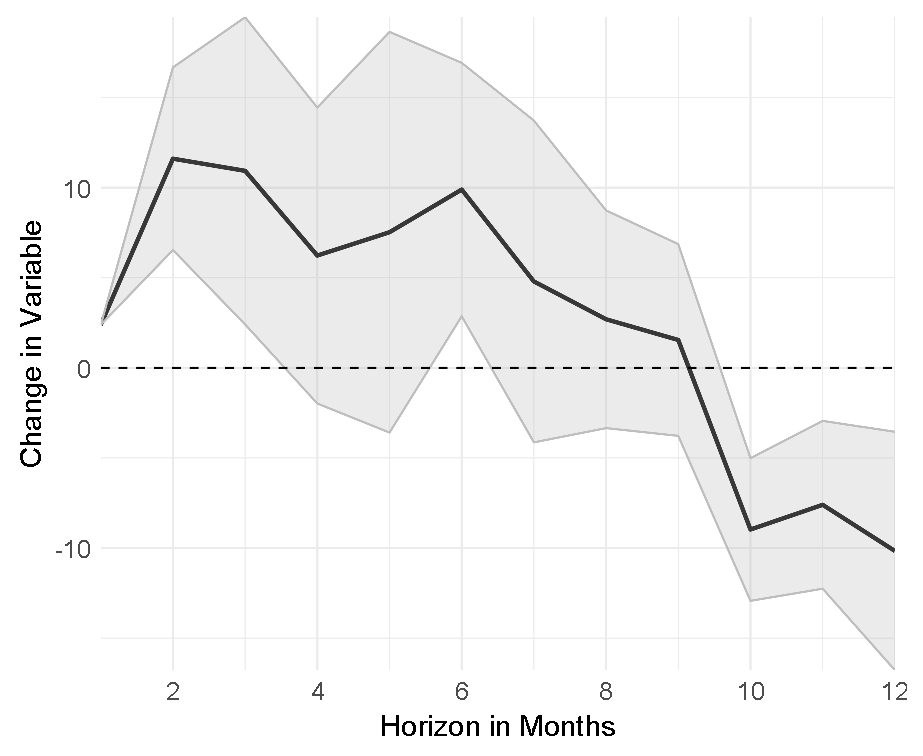
\includegraphics[width=0.8\textwidth]{output/lp/baseline/bHP/supply_chain/supply_chainonexpectations1y_djn.eps}
		\caption{Supply chain on 1-year expectations}
	\end{subfigure}
	\begin{subfigure}{00.24\textwidth}
		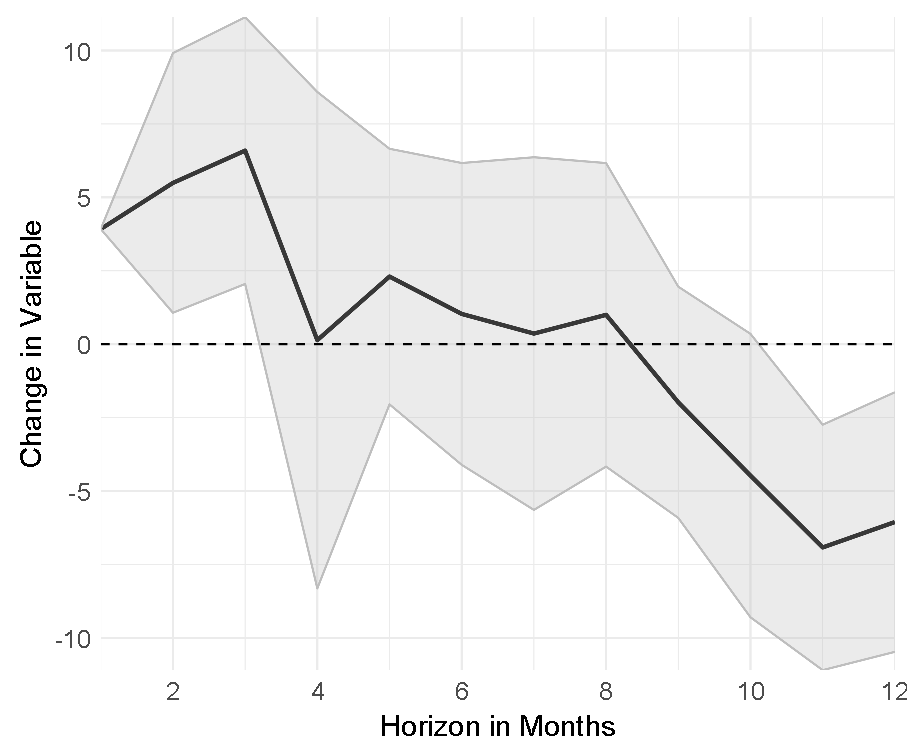
\includegraphics[width=0.8\textwidth]{output/lp/baseline/bHP/supply_chain/supply_chainonexpectations3y_djn.eps}
		\caption{Supply chain on 3-year expectations}
	\end{subfigure}
	\begin{subfigure}{00.24\textwidth}
		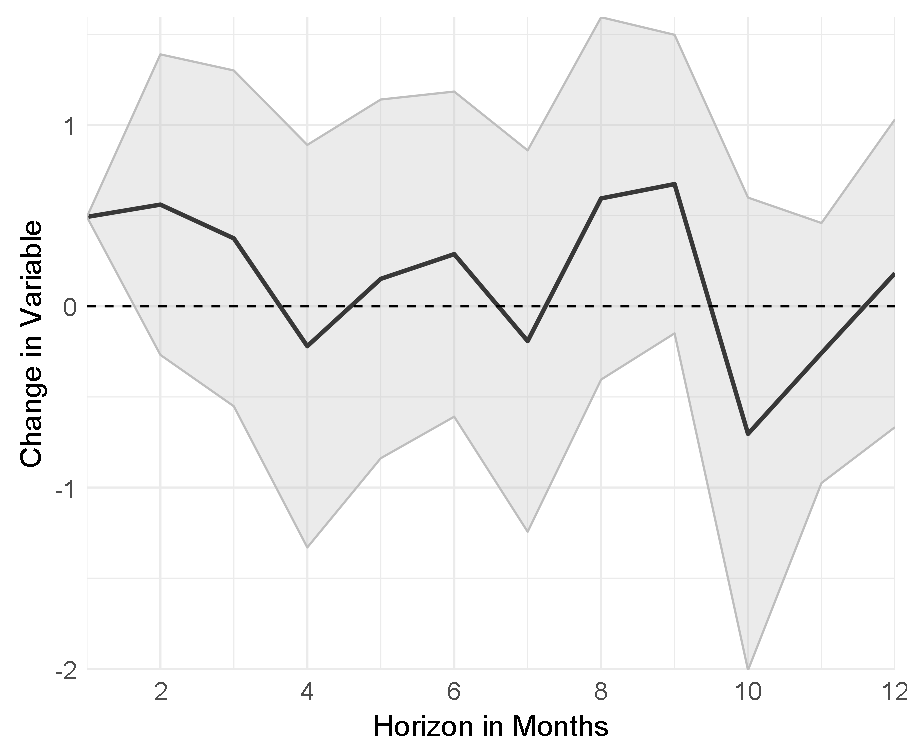
\includegraphics[width=0.8\textwidth]{output/lp/baseline/bHP/supply_chain/supply_chainoninflation_djn.eps}
		\caption{Supply chain on CPI inflation}
	\end{subfigure}
	\begin{subfigure}{00.24\textwidth}
		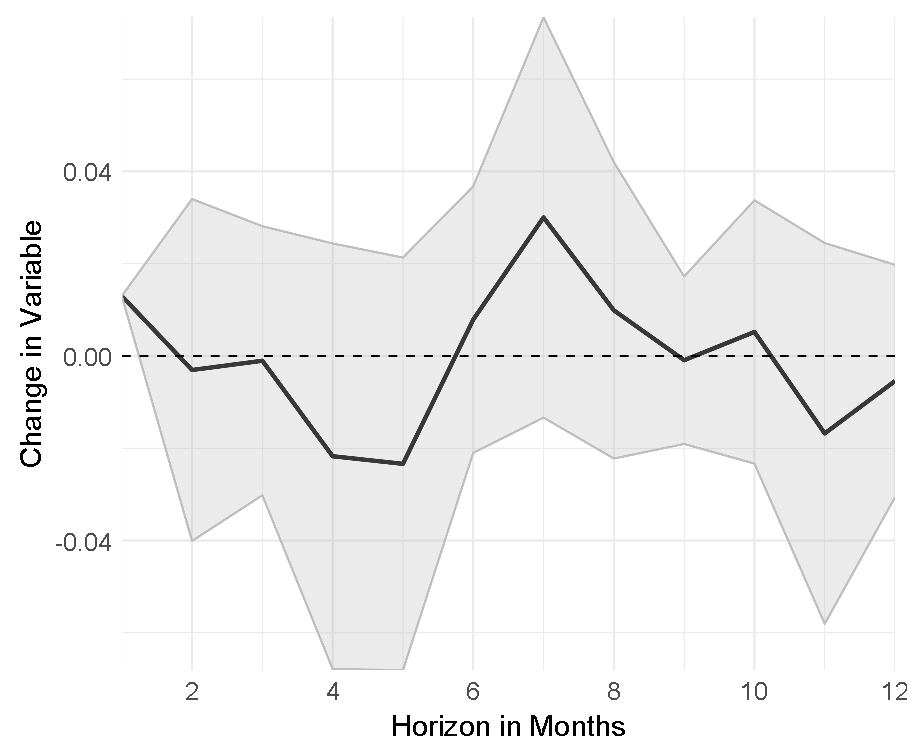
\includegraphics[width=0.8\textwidth]{output/lp/baseline/bHP/supply_chain/supply_chainoneconac_djn.eps}
		\caption{Supply chain on economic activity}
	\end{subfigure}
	\begin{subfigure}{00.24\textwidth}
		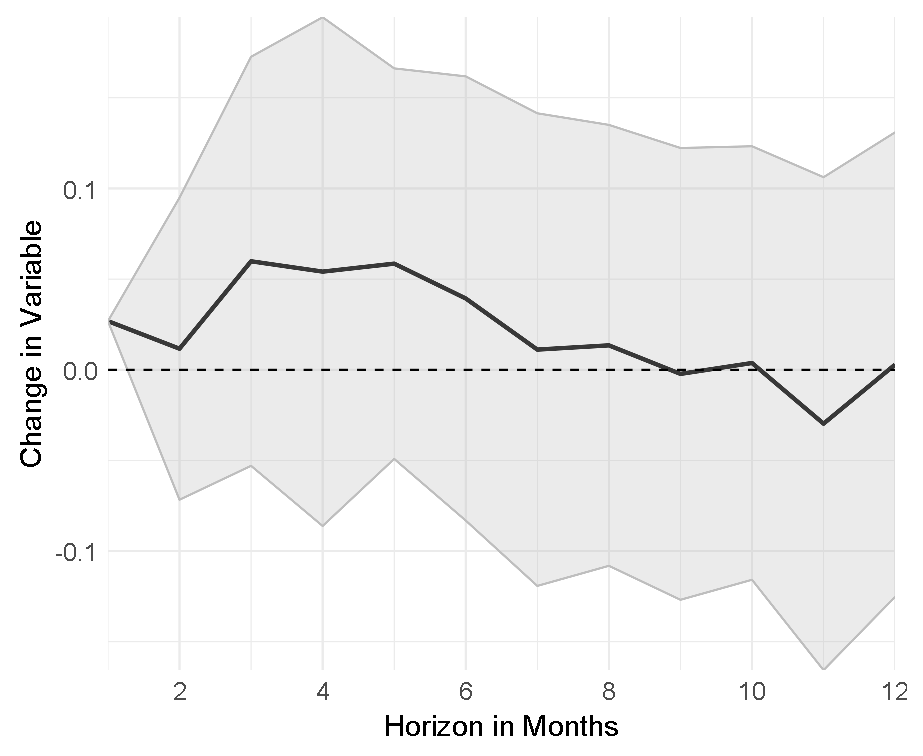
\includegraphics[width=0.8\textwidth]{output/lp/baseline/bHP/energy/energyonexpectations1y_djn.eps}
		\caption{Energy on 1-year expectations}
	\end{subfigure}
	\begin{subfigure}{00.24\textwidth}
		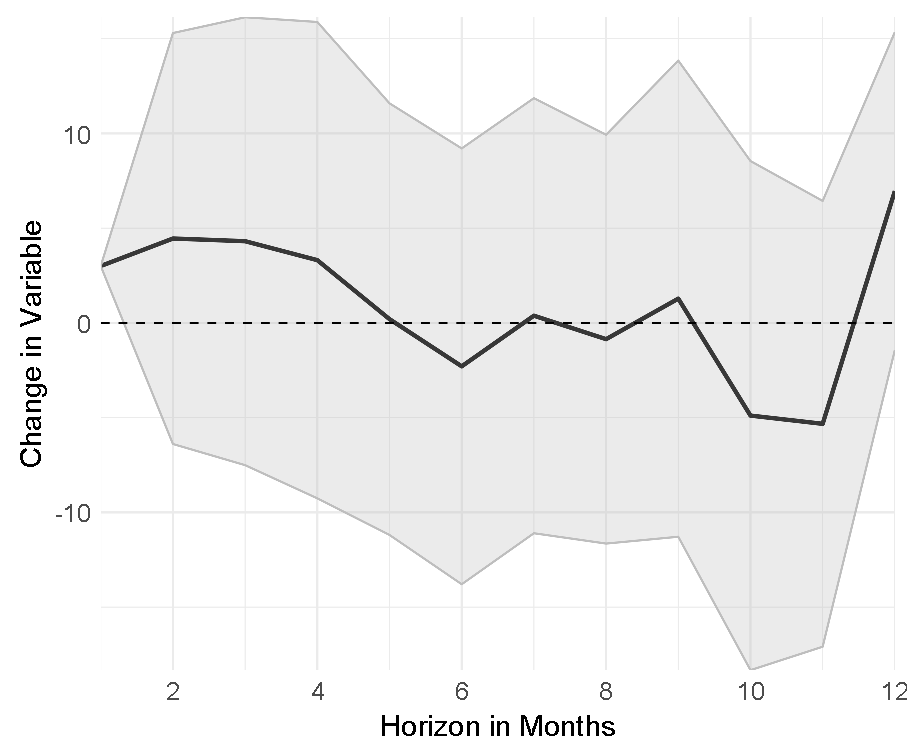
\includegraphics[width=0.8\textwidth]{output/lp/baseline/bHP/energy/energyonexpectations3y_djn.eps}
		\caption{Energy on 3-year expectations}
	\end{subfigure}
	\begin{subfigure}{00.24\textwidth}
		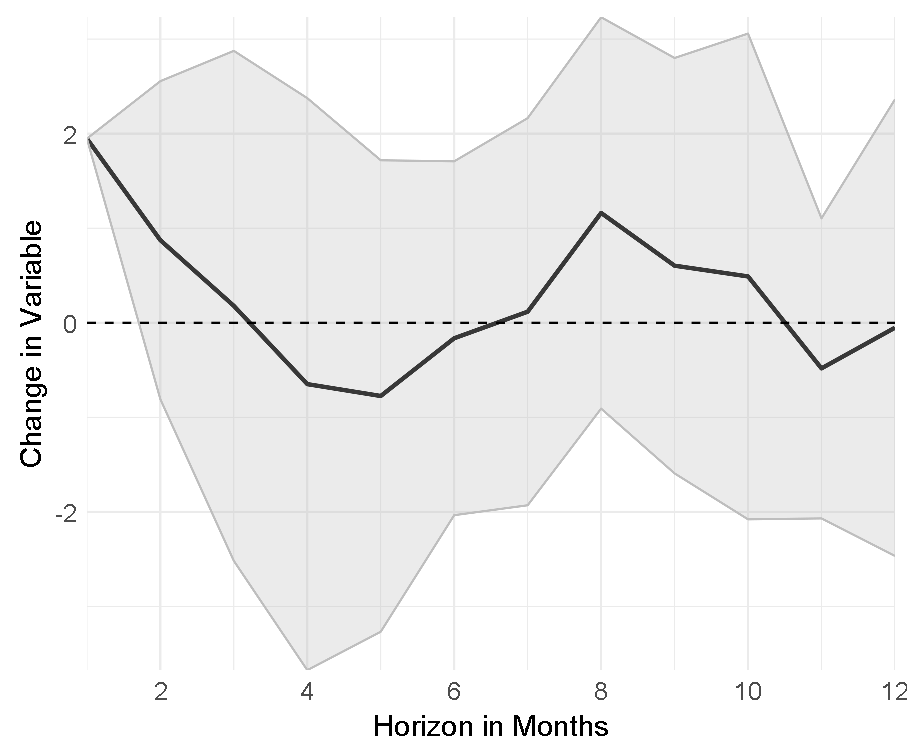
\includegraphics[width=0.8\textwidth]{output/lp/baseline/bHP/energy/energyoninflation_djn.eps}
		\caption{Energy on CPI inflation}
	\end{subfigure}
	\begin{subfigure}{00.24\textwidth}
		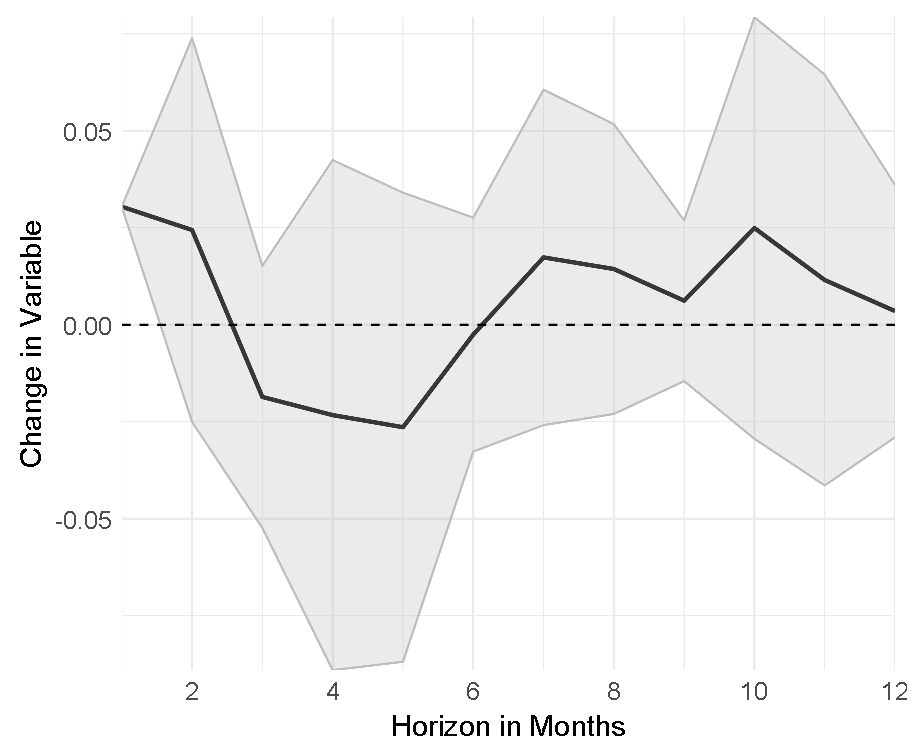
\includegraphics[width=0.8\textwidth]{output/lp/baseline/bHP/energy/energyoneconac_djn.eps}
		\caption{Energy on economic activity}
	\end{subfigure}
	\begin{subfigure}{00.24\textwidth}
		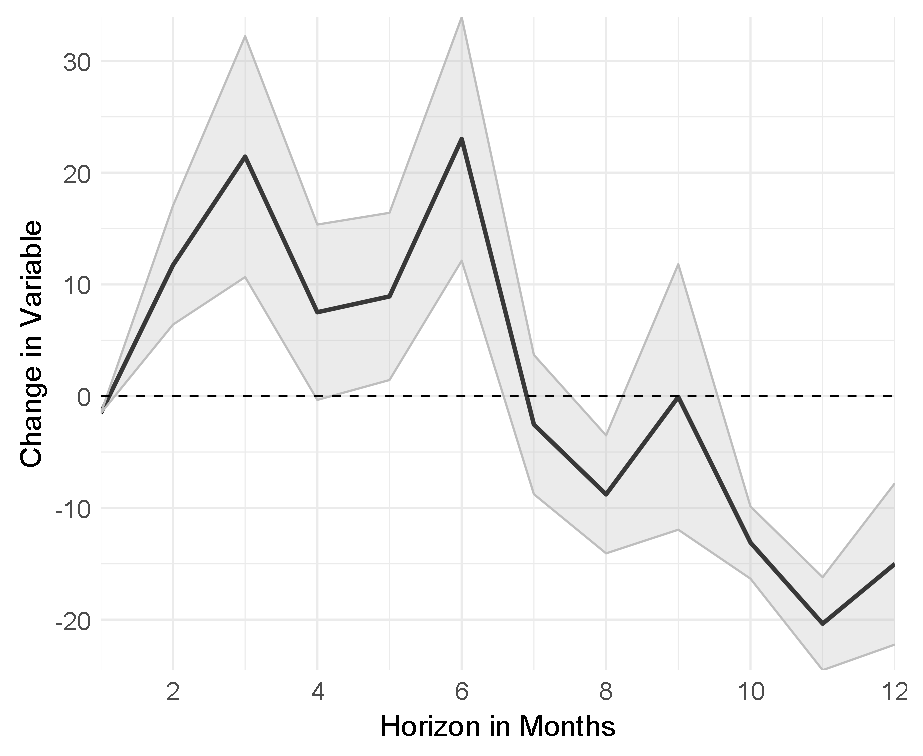
\includegraphics[width=0.8\textwidth]{output/lp/baseline/bHP/labor_shortage/labor_shortageonexpectations1y_djn.eps}
		\caption{Labor shortage on 1-year expectations}
	\end{subfigure}
	\begin{subfigure}{00.24\textwidth}
		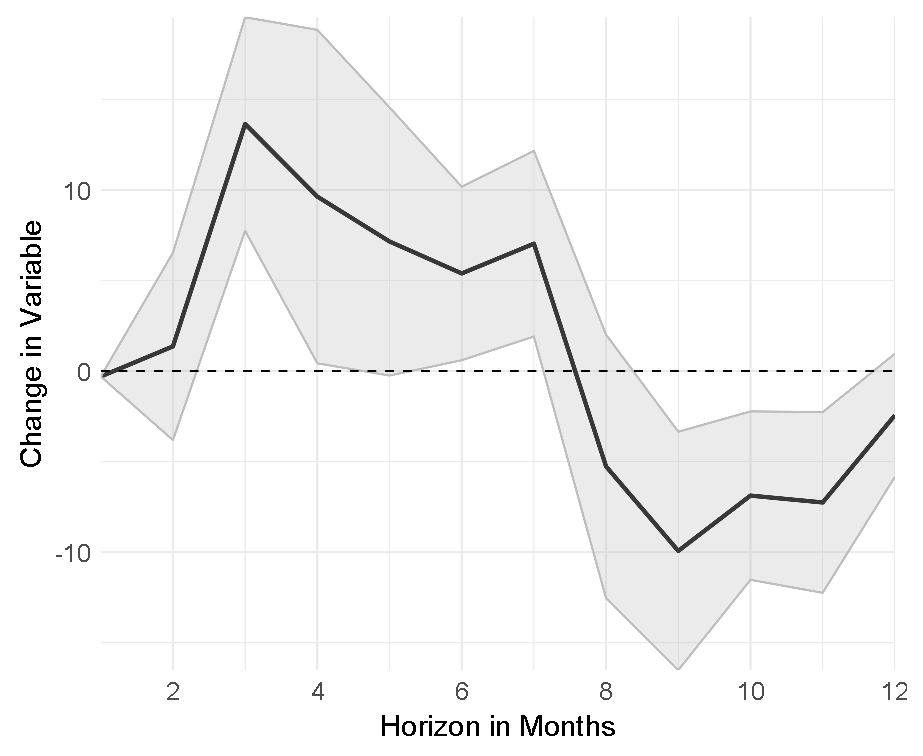
\includegraphics[width=0.8\textwidth]{output/lp/baseline/bHP/labor_shortage/labor_shortageonexpectations3y_djn.eps}
		\caption{Labor shortage on 3-year expectations}
	\end{subfigure}
	\begin{subfigure}{00.24\textwidth}
		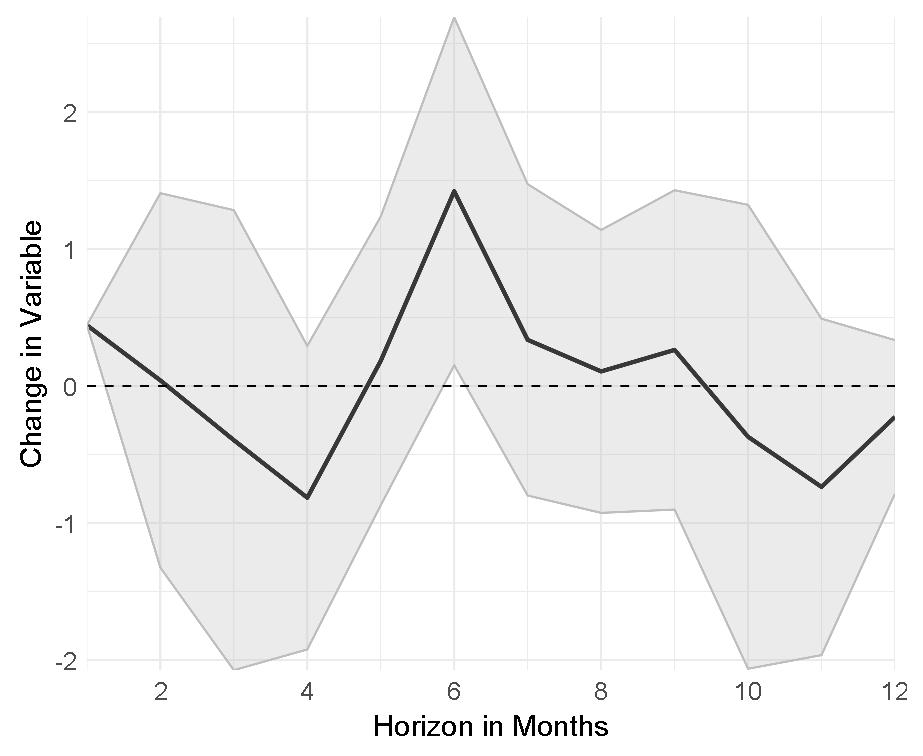
\includegraphics[width=0.8\textwidth]{output/lp/baseline/bHP/labor_shortage/labor_shortageoninflation_djn.eps}
		\caption{Labor shortage on CPI inflation}
	\end{subfigure}
	\begin{subfigure}{00.24\textwidth}
		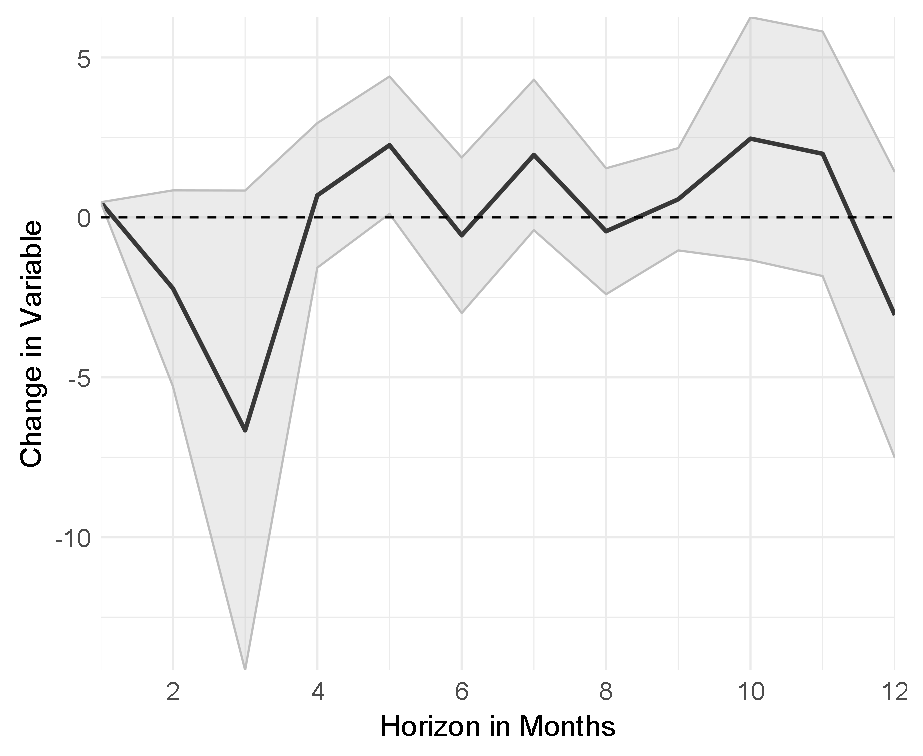
\includegraphics[width=0.8\textwidth]{output/lp/baseline/bHP/labor_shortage/labor_shortageoneconac_djn.eps}
		\caption{Labor shortage on economic activity}
	\end{subfigure}
		\begin{subfigure}{00.24\textwidth}
		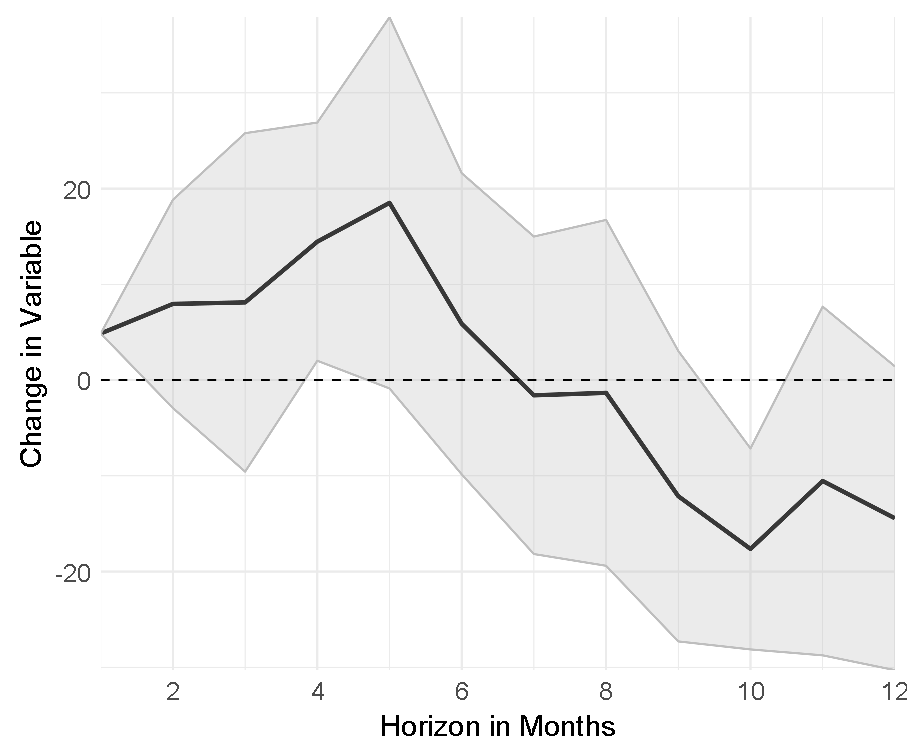
\includegraphics[width=0.8\textwidth]{output/lp/baseline/bHP/supply/supplyonexpectations1y_djn.eps}
		\caption{Supply (residual) on 1-year expectations}
	\end{subfigure}
	\begin{subfigure}{00.24\textwidth}
		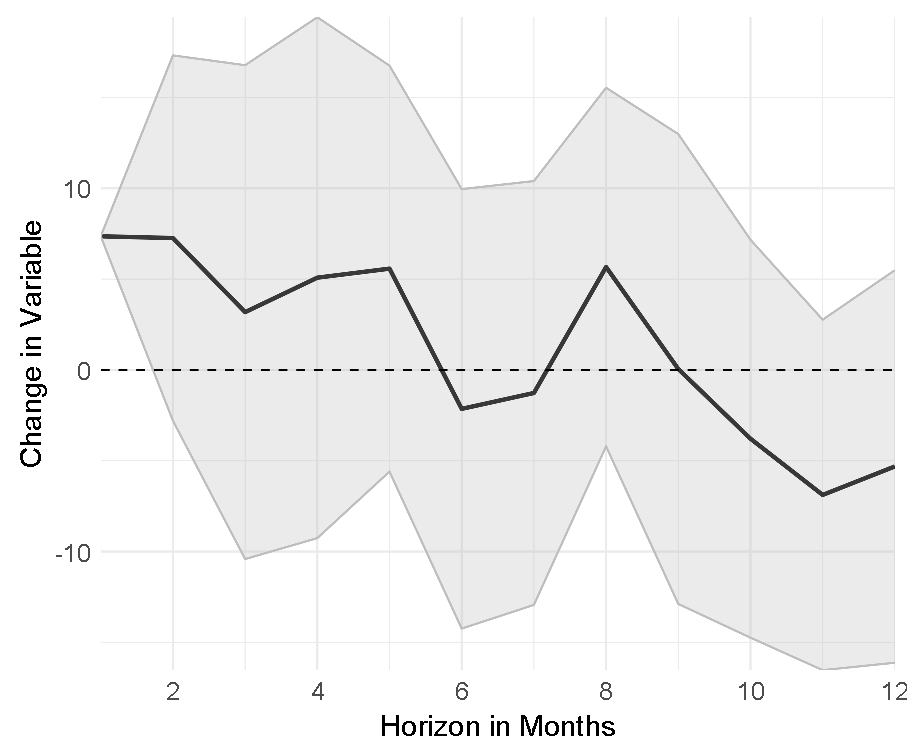
\includegraphics[width=0.8\textwidth]{output/lp/baseline/bHP/supply/supplyonexpectations3y_djn.eps}
		\caption{Supply (residual) on 3-year expectations}
	\end{subfigure}
	\begin{subfigure}{00.24\textwidth}
		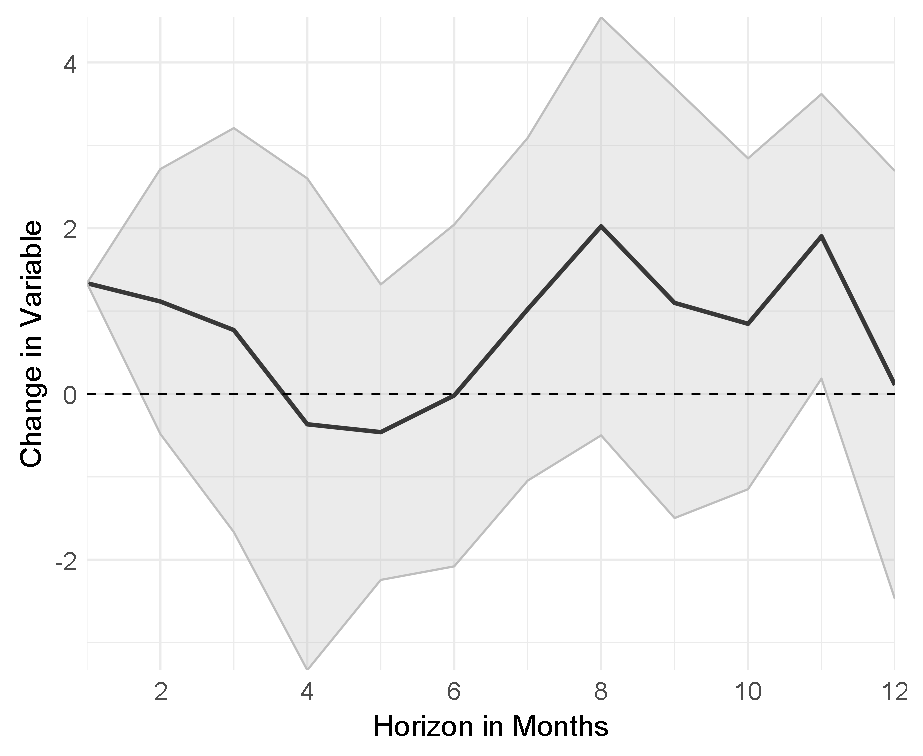
\includegraphics[width=0.8\textwidth]{output/lp/baseline/bHP/supply/supplyoninflation_djn.eps}
		\caption{Supply (residual) on CPI inflation}
	\end{subfigure}
	\begin{subfigure}{00.24\textwidth}
		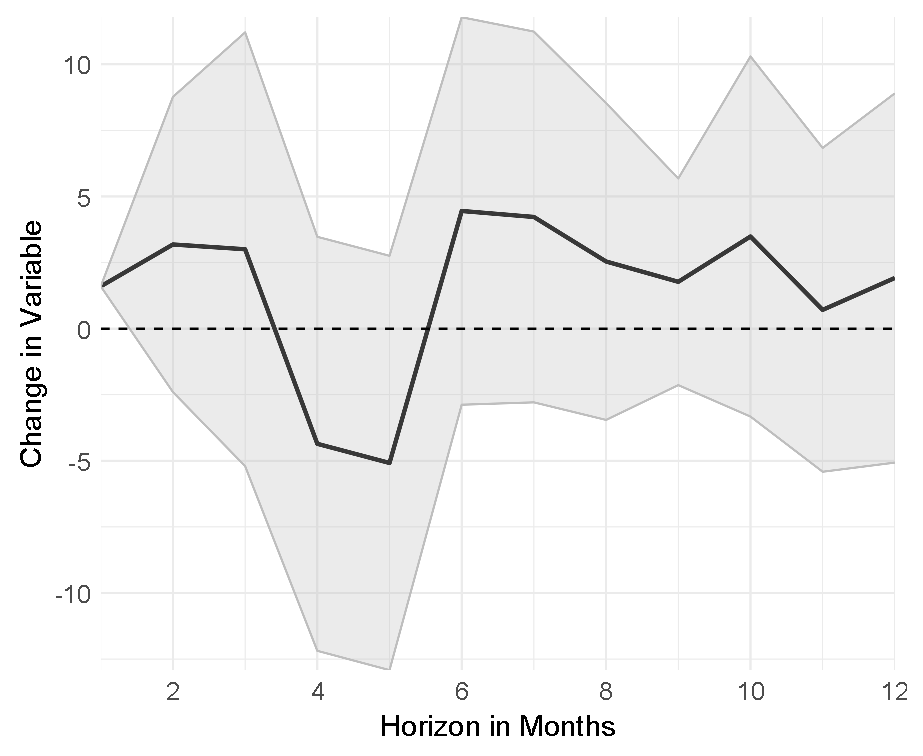
\includegraphics[width=0.8\textwidth]{output/lp/baseline/bHP/supply/supplyoneconac_djn.eps}
		\caption{Supply (residual) on economic activity}
	\end{subfigure}
	\caption{Supply narratives' impulse responses}
	\label{fig:irf_2}
\end{sidewaysfigure}

\newpage
\begin{sidewaysfigure}[H]
	\centering
	\captionsetup{font=footnotesize}
	\begin{subfigure}{00.24\textwidth}
		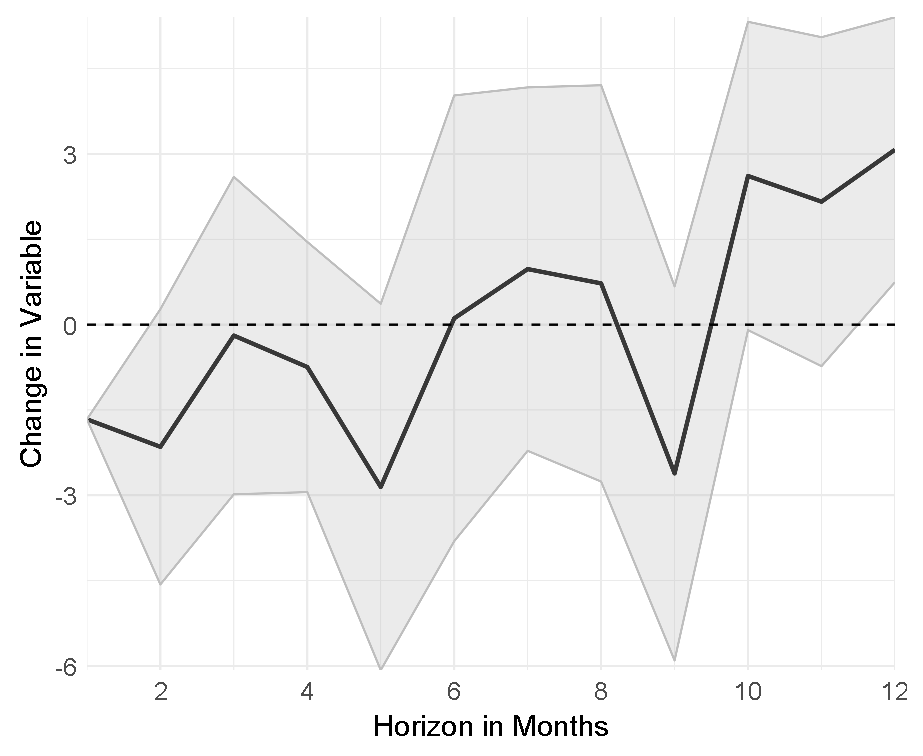
\includegraphics[width=0.8\textwidth]{output/lp/baseline/bHP/pandemic/pandemiconexpectations1y_djn.eps}
		\caption{Pandemic on 1-year expectations}
	\end{subfigure}
	\begin{subfigure}{00.24\textwidth}
		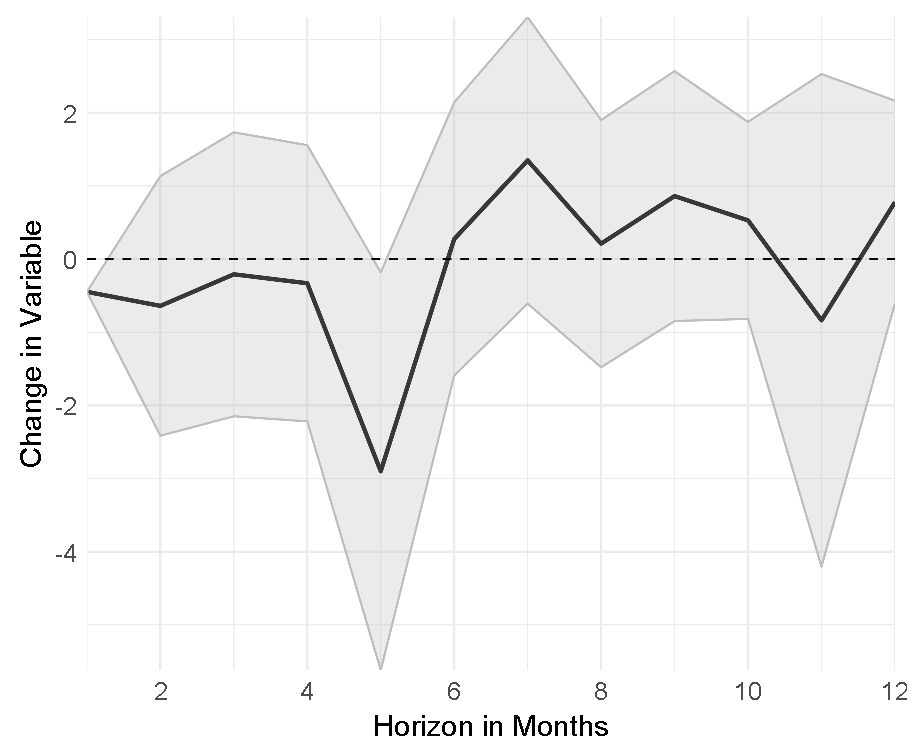
\includegraphics[width=0.8\textwidth]{output/lp/baseline/bHP/pandemic/pandemiconexpectations3y_djn.eps}
		\caption{Pandemic on 3-year expectations}
	\end{subfigure}
	\begin{subfigure}{00.24\textwidth}
		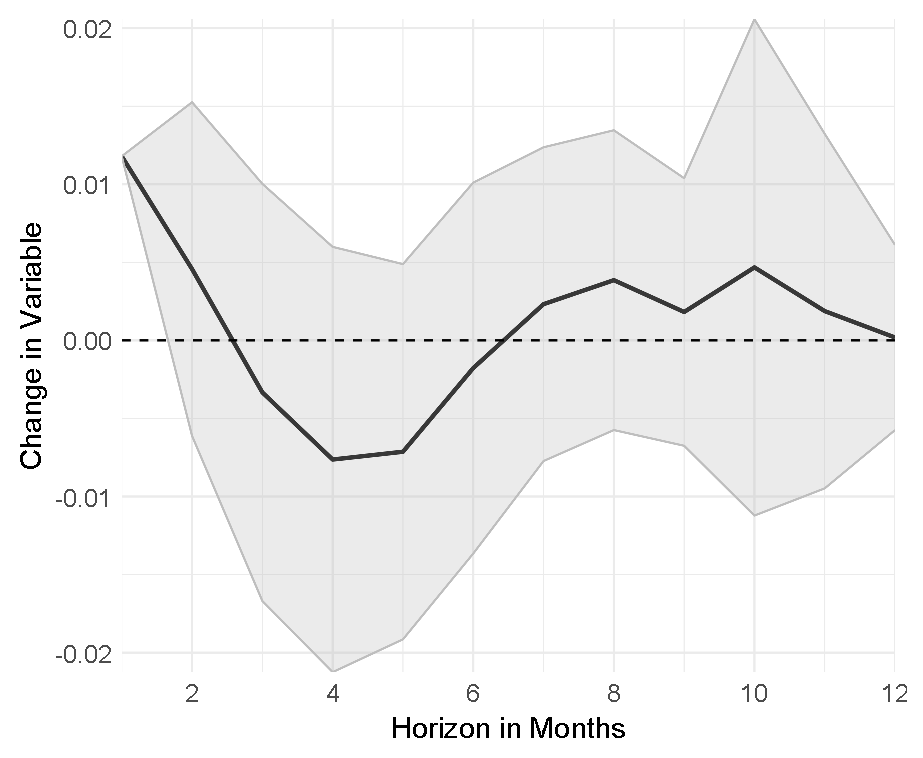
\includegraphics[width=0.8\textwidth]{output/lp/baseline/bHP/pandemic/pandemiconinflation_djn.eps}
		\caption{Pandemic on CPI inflation}
	\end{subfigure}
	\begin{subfigure}{00.24\textwidth}
		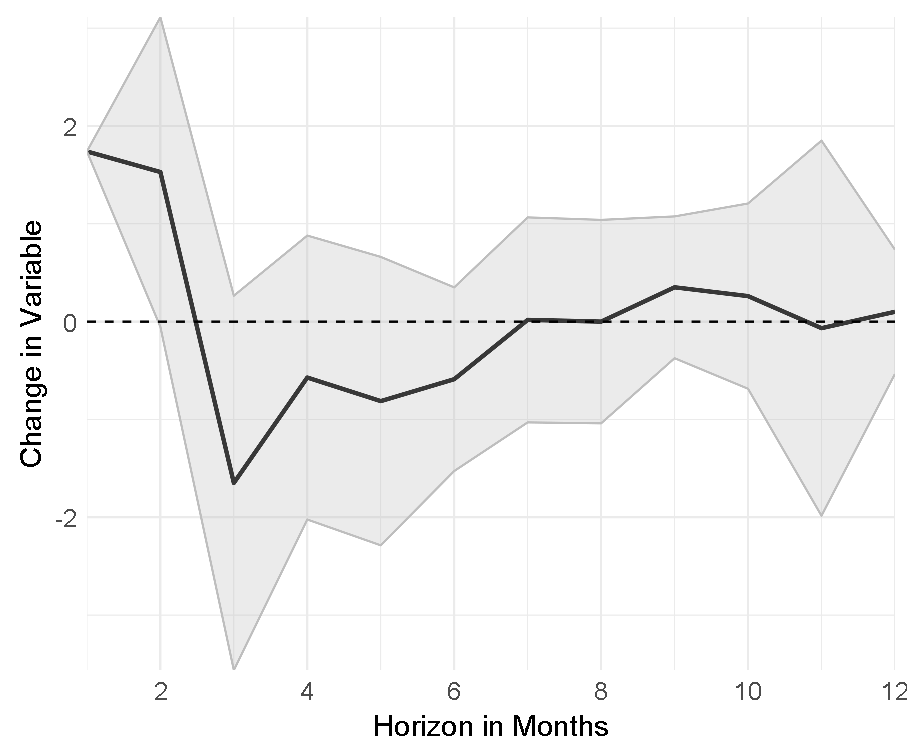
\includegraphics[width=0.8\textwidth]{output/lp/baseline/bHP/pandemic/pandemiconeconac_djn.eps}
		\caption{Pandemic on economic activity}
	\end{subfigure}
	\begin{subfigure}{00.24\textwidth}
		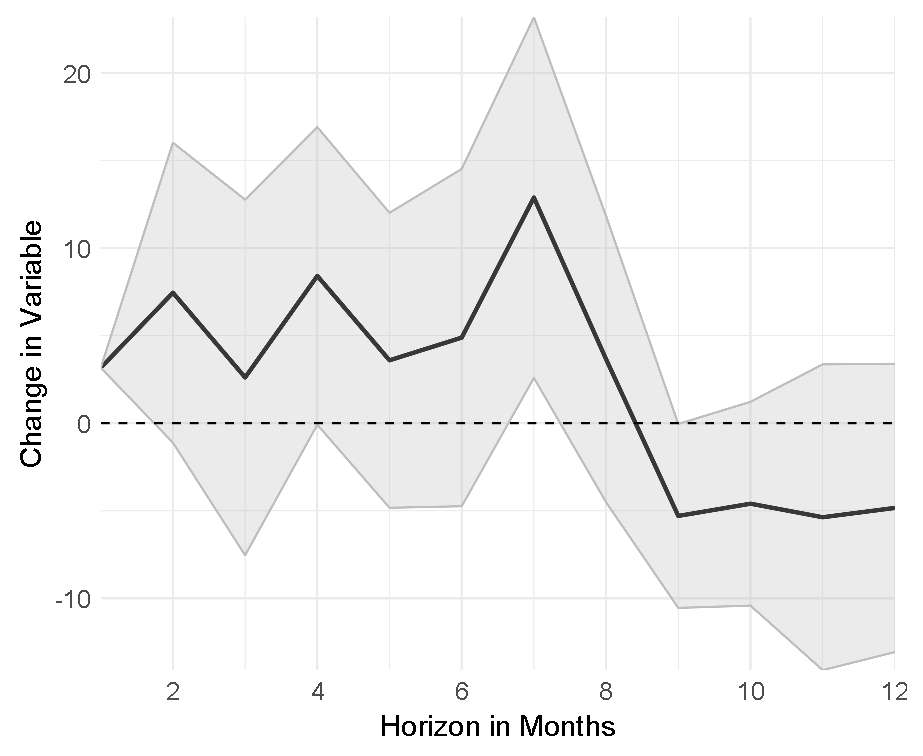
\includegraphics[width=0.8\textwidth]{output/lp/baseline/bHP/politics/politicsonexpectations1y_djn.eps}
		\caption{Politics on 1-year expectations}
	\end{subfigure}
	\begin{subfigure}{00.24\textwidth}
		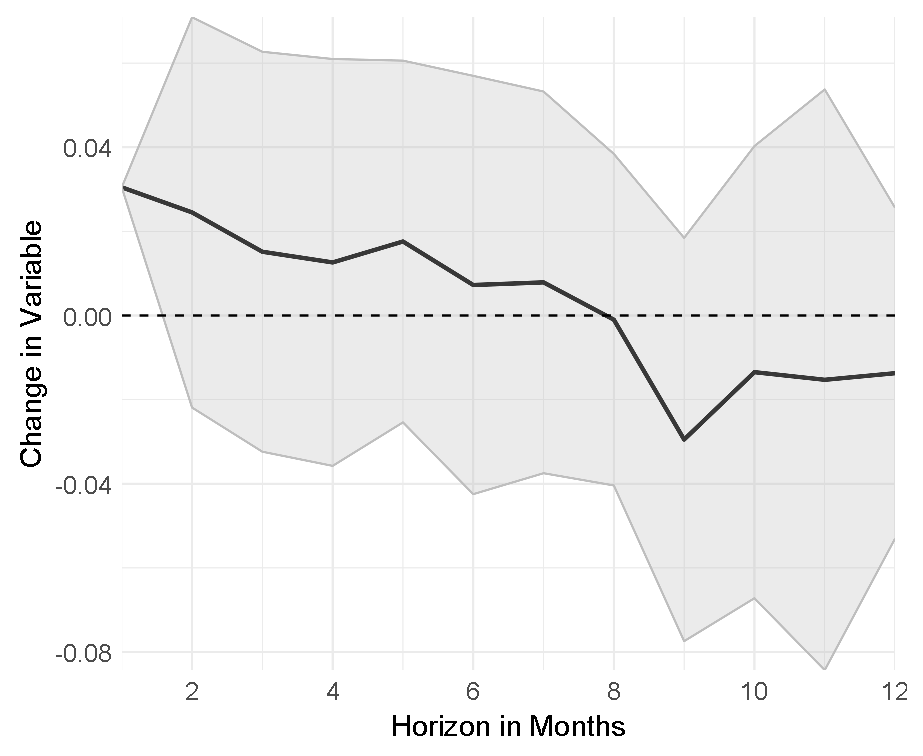
\includegraphics[width=0.8\textwidth]{output/lp/baseline/bHP/politics/politicsonexpectations3y_djn.eps}
		\caption{Politics on 3-year expectations}
	\end{subfigure}
	\begin{subfigure}{00.24\textwidth}
		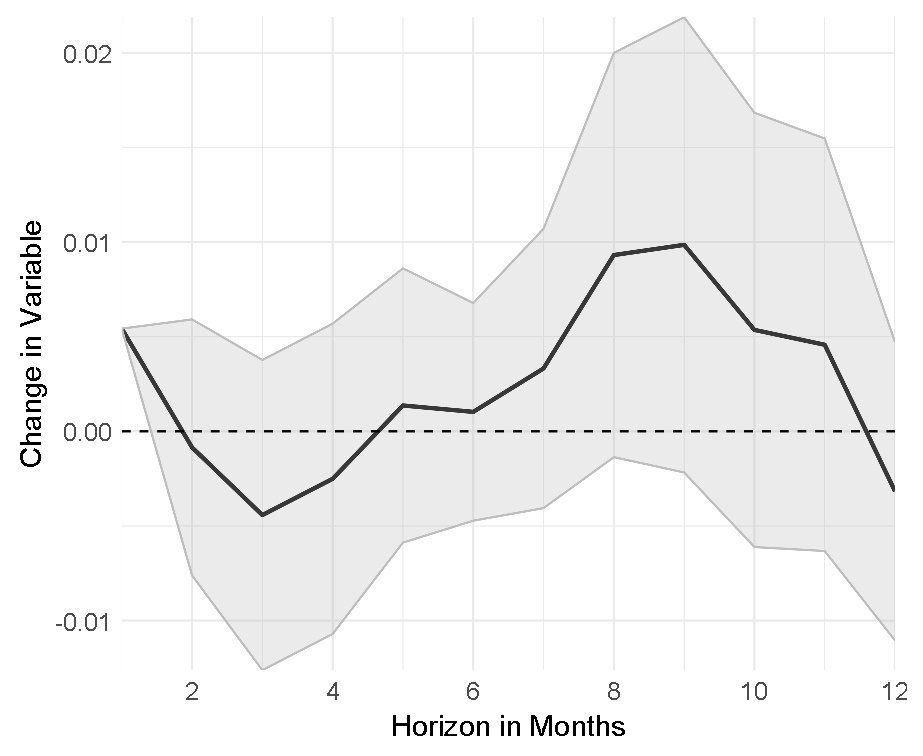
\includegraphics[width=0.8\textwidth]{output/lp/baseline/bHP/politics/politicsoninflation_djn.eps}
		\caption{Politics on CPI inflation}
	\end{subfigure}
	\begin{subfigure}{00.24\textwidth}
		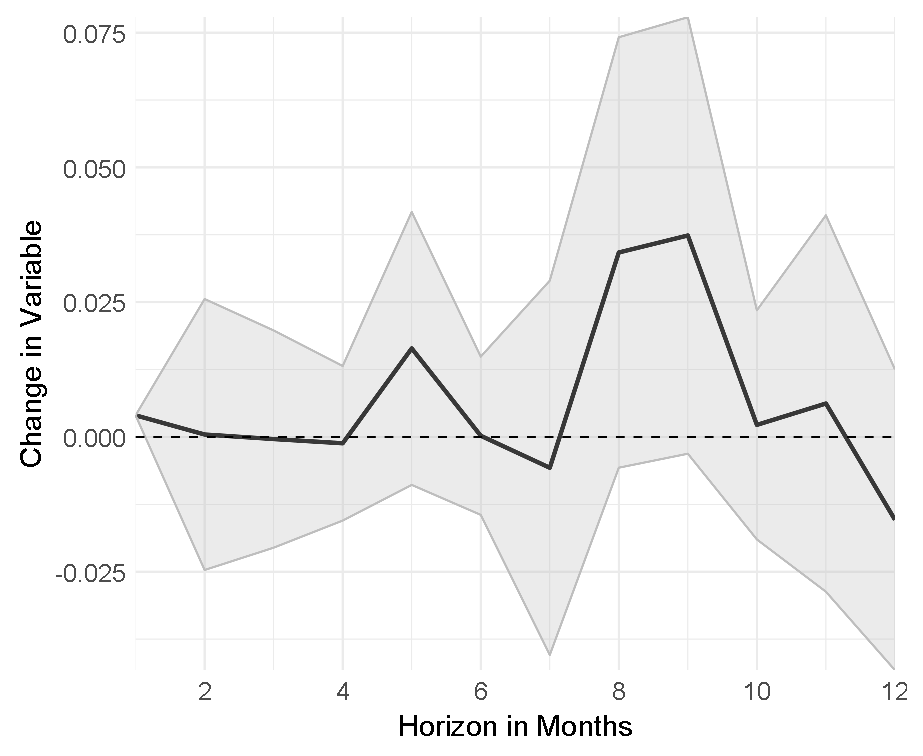
\includegraphics[width=0.8\textwidth]{output/lp/baseline/bHP/politics/politicsoneconac_djn.eps}
		\caption{Politics on economic activity}
	\end{subfigure}
	\begin{subfigure}{00.24\textwidth}
		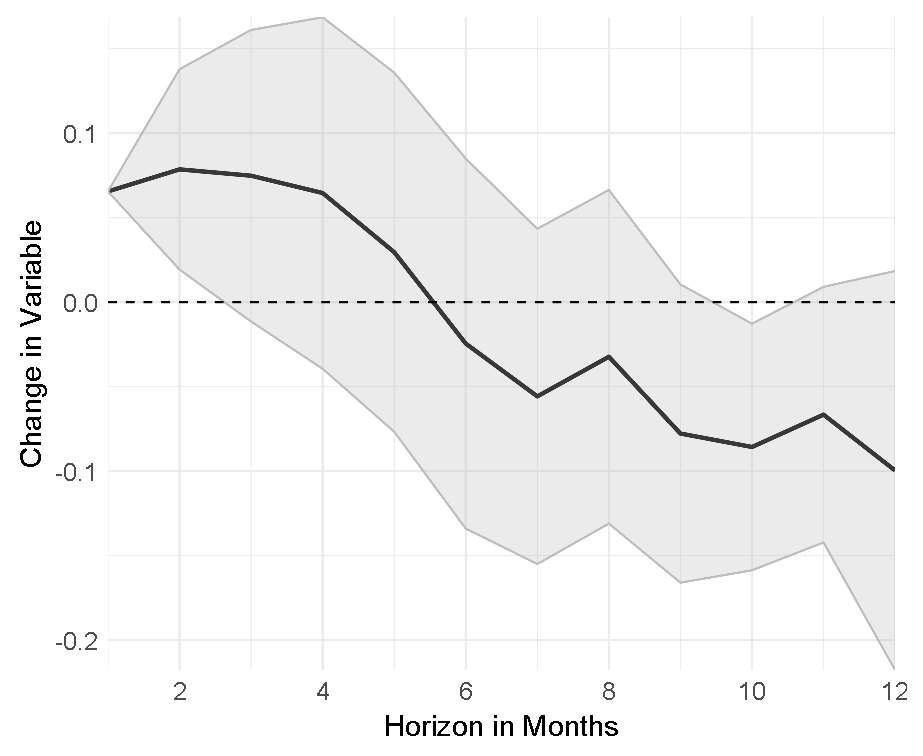
\includegraphics[width=0.8\textwidth]{output/lp/baseline/bHP/war/waronexpectations1y_djn.eps}
		\caption{War on 1-year expectations}
	\end{subfigure}
	\begin{subfigure}{00.24\textwidth}
		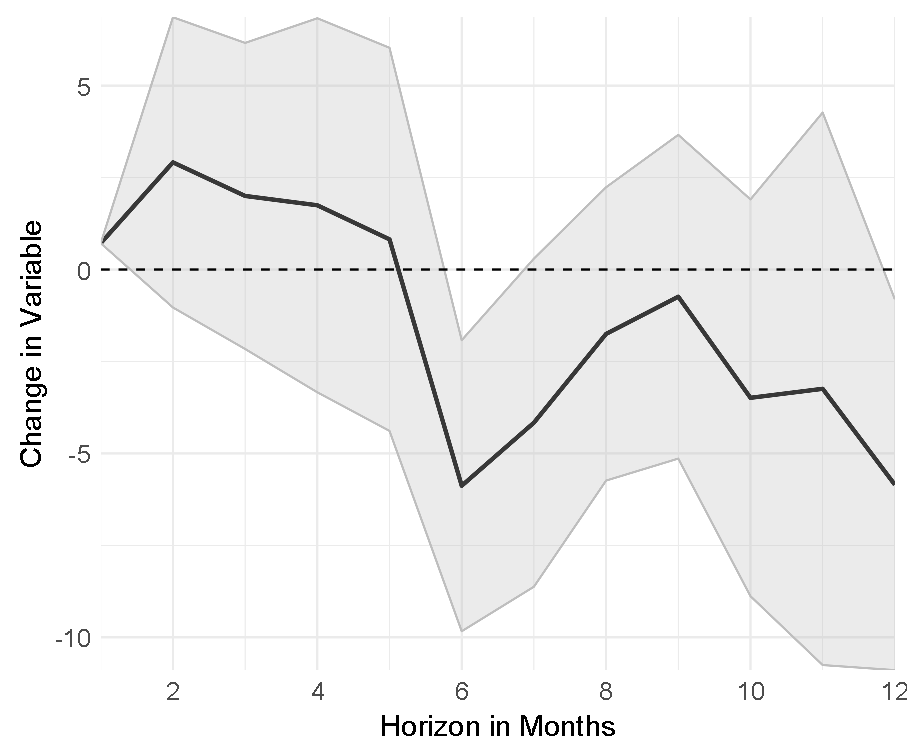
\includegraphics[width=0.8\textwidth]{output/lp/baseline/bHP/war/waronexpectations3y_djn.eps}
		\caption{War on 3-year expectations}
	\end{subfigure}
	\begin{subfigure}{00.24\textwidth}
		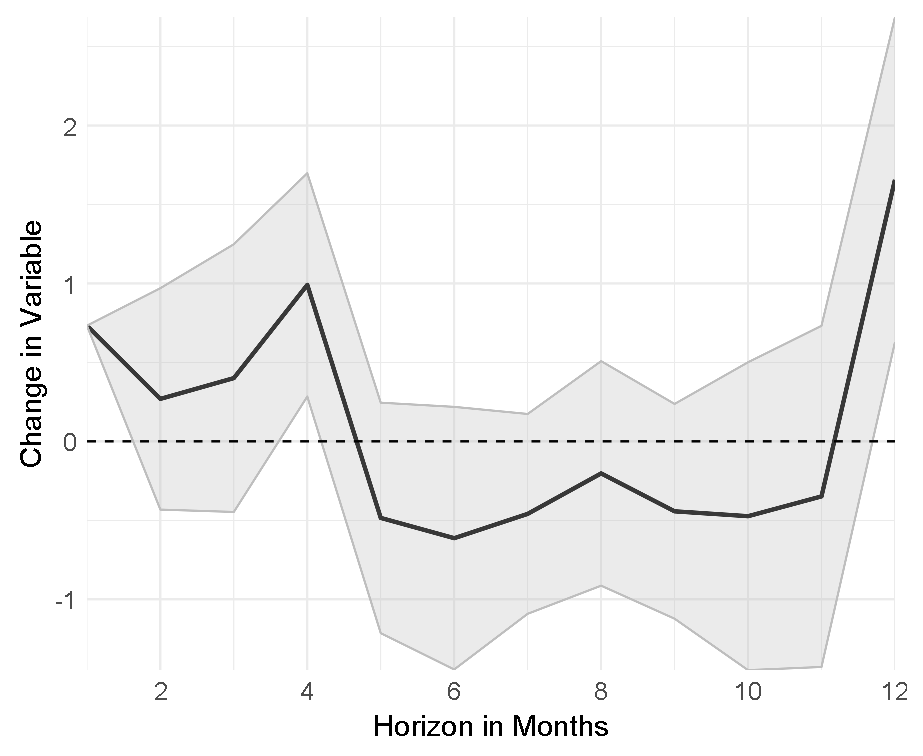
\includegraphics[width=0.8\textwidth]{output/lp/baseline/bHP/war/waroninflation_djn.eps}
		\caption{War on CPI inflation}
	\end{subfigure}
	\begin{subfigure}{00.24\textwidth}
		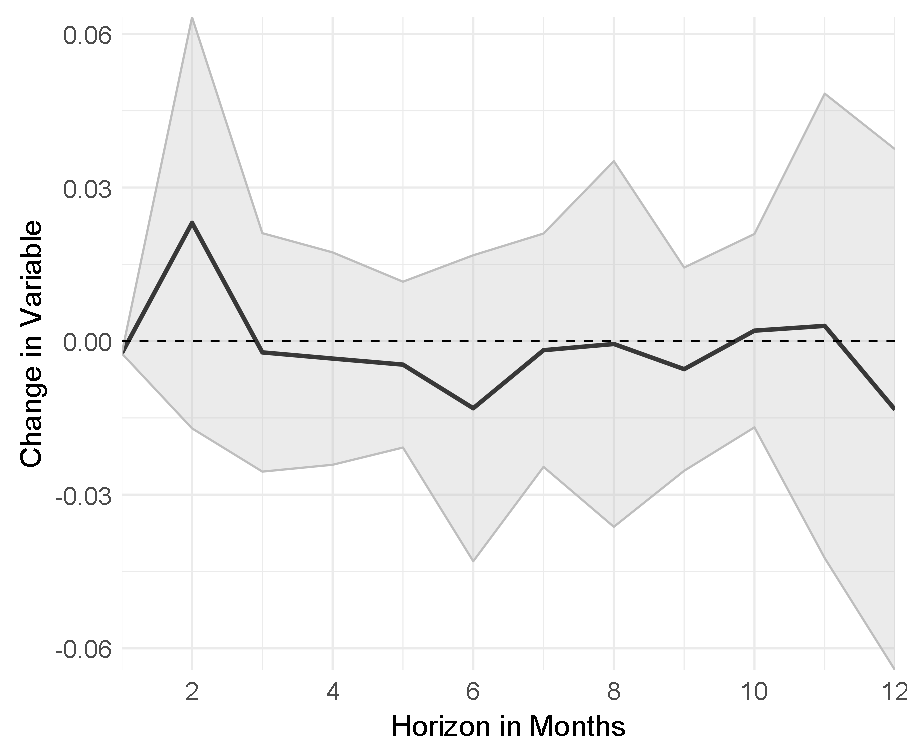
\includegraphics[width=0.8\textwidth]{output/lp/baseline/bHP/war/waroneconac_djn.eps}
		\caption{War on economic activity}
	\end{subfigure}
	\begin{subfigure}{00.24\textwidth}
		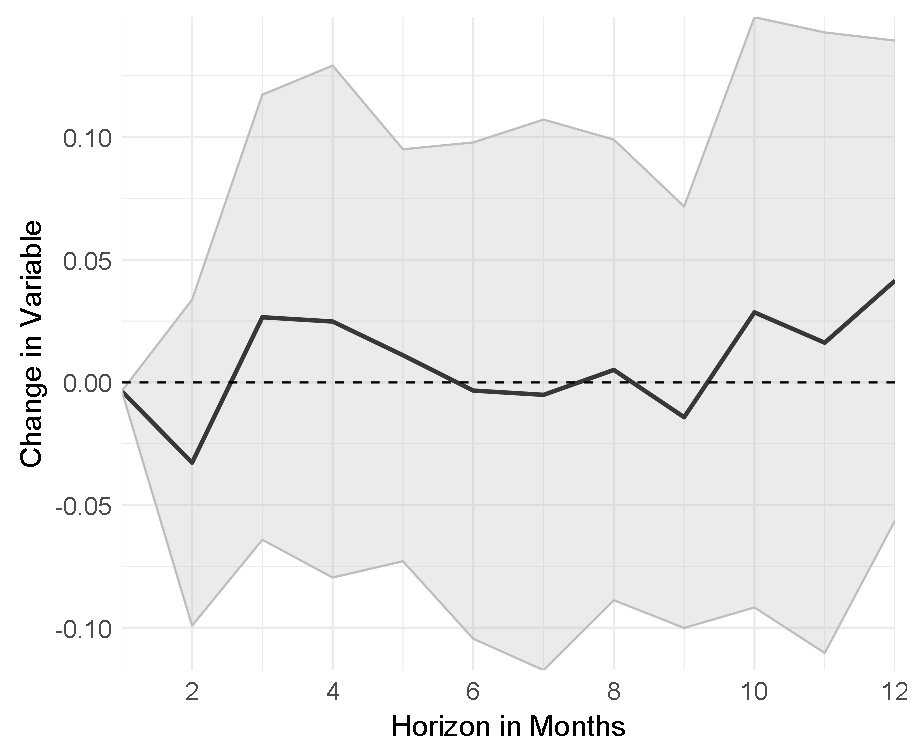
\includegraphics[width=0.8\textwidth]{output/lp/baseline/bHP/debt/debtonexpectations1y_djn.eps}
		\caption{Debt on 1-year expectations}
	\end{subfigure}
	\begin{subfigure}{00.24\textwidth}
		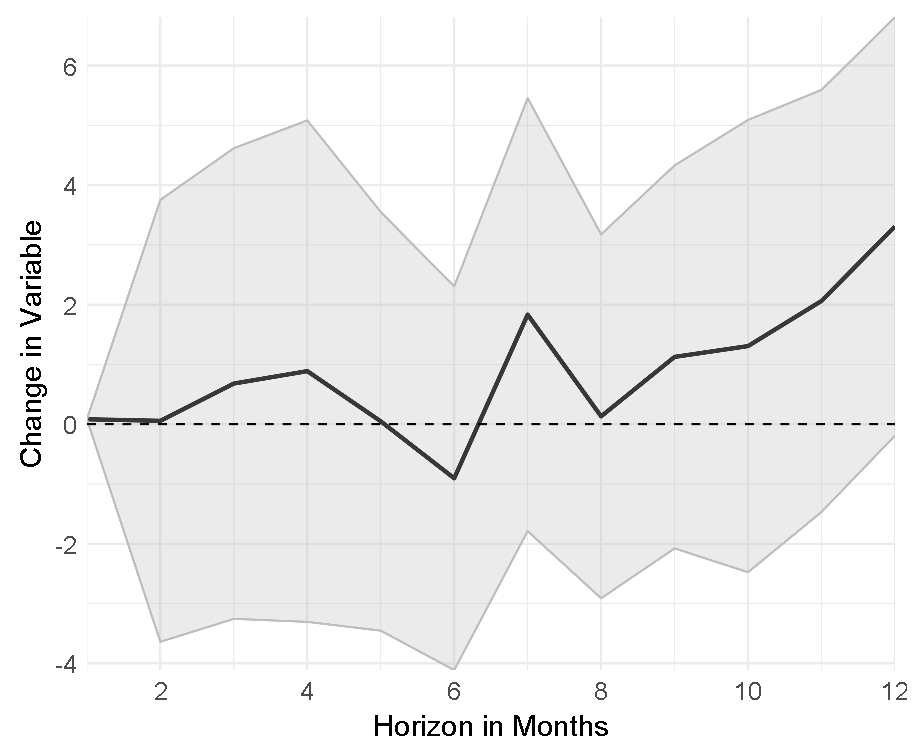
\includegraphics[width=0.8\textwidth]{output/lp/baseline/bHP/debt/debtonexpectations3y_djn.eps}
		\caption{Debt on 3-year expectations}
	\end{subfigure}
	\begin{subfigure}{00.24\textwidth}
		\includegraphics[width=0.8\textwidth]{output/lp/baseline/bHP/debt/debtoninflation_djn.eps}
		\caption{Debt on CPI inflation}
	\end{subfigure}
	\begin{subfigure}{00.24\textwidth}
		\includegraphics[width=0.8\textwidth]{output/lp/baseline/bHP/debt/debtoneconac_djn.eps}
		\caption{Debt on economic activity}
	\end{subfigure}
	\caption{Miscellaneous narratives' impulse responses}
	\label{fig:irf_3}
\end{sidewaysfigure}

\newpage
\begin{sidewaysfigure}[H]
	\centering
	\captionsetup{font=footnotesize}
	\begin{subfigure}{00.24\textwidth}
		\includegraphics[width=0.8\textwidth]{output/lp/baseline/bHP/taxes/taxesonexpectations1y_djn.eps}
		\caption{Taxes on 1-year expectations}
	\end{subfigure}
	\begin{subfigure}{00.24\textwidth}
		\includegraphics[width=0.8\textwidth]{output/lp/baseline/bHP/taxes/taxesonexpectations3y_djn.eps}
		\caption{Taxes on 3-year expectations}
	\end{subfigure}
	\begin{subfigure}{00.24\textwidth}
		\includegraphics[width=0.8\textwidth]{output/lp/baseline/bHP/taxes/taxesoninflation_djn.eps}
		\caption{Taxes on CPI inflation}
	\end{subfigure}
	\begin{subfigure}{00.24\textwidth}
		\includegraphics[width=0.8\textwidth]{output/lp/baseline/bHP/taxes/taxesoneconac_djn.eps}
		\caption{Taxes on economic activity}
	\end{subfigure}
	\begin{subfigure}{00.24\textwidth}
		\includegraphics[width=0.8\textwidth]{output/lp/baseline/bHP/profits/profitsonexpectations1y_djn.eps}
		\caption{Profits on 1-year expectations}
	\end{subfigure}
	\begin{subfigure}{00.24\textwidth}
		\includegraphics[width=0.8\textwidth]{output/lp/baseline/bHP/profits/profitsonexpectations3y_djn.eps}
		\caption{Profits on 3-year expectations}
	\end{subfigure}
	\begin{subfigure}{00.24\textwidth}
		\includegraphics[width=0.8\textwidth]{output/lp/baseline/bHP/profits/profitsoninflation_djn.eps}
		\caption{Profits on CPI inflation}
	\end{subfigure}
	\begin{subfigure}{00.24\textwidth}
		\includegraphics[width=0.8\textwidth]{output/lp/baseline/bHP/profits/profitsoneconac_djn.eps}
		\caption{Profits on economic activity}
	\end{subfigure}
	\caption{Miscellaneous narratives' impulse responses (bHP)}
	\label{fig:irf_4}
\end{sidewaysfigure}



\newpage

%Robustness IRF



\begin{figure}[H]
	\centering
	\captionsetup{font=footnotesize}
	\begin{subfigure}{00.32\textwidth}
	\includegraphics[width=1\textwidth]{output/lp/baseline/level/government_spending/government_spendingonexpectations1y_djn.eps}
	\caption{Government spending on 1-year}
\end{subfigure}
\begin{subfigure}{00.32\textwidth}
	\includegraphics[width=1\textwidth]{output/lp/baseline/level/monetary_policy/monetary_policyonexpectations3y_djn.eps}
	\caption{Monetary policy on 3-year}
\end{subfigure}
\begin{subfigure}{00.32\textwidth}
	\includegraphics[width=1\textwidth]{output/lp/baseline/level/supply_chain/supply_chainonexpectations1y_djn.eps}
	\caption{Supply chain on 1-year}
\end{subfigure}
\begin{subfigure}{00.32\textwidth}
	\includegraphics[width=1\textwidth]{output/lp/baseline/level/pandemic/pandemiconexpectations1y_djn.eps}
	\caption{Pandemic on 1-year}
\end{subfigure}
\begin{subfigure}{00.32\textwidth}
	\includegraphics[width=1\textwidth]{output/lp/baseline/level/politics/politicsonexpectations3y_djn.eps}
	\caption{Politics on 3-year}
\end{subfigure}
\begin{subfigure}{00.32\textwidth}
	\includegraphics[width=1\textwidth]{output/lp/baseline/level/war/waronexpectations1y_djn.eps}
	\caption{War on 1-year}
\end{subfigure}
\begin{subfigure}{00.32\textwidth}
	\includegraphics[width=1\textwidth]{output/lp/baseline/level/war/waronexpectations3y_djn.eps}
	\caption{War on 3-year}
\end{subfigure}
\begin{subfigure}{00.32\textwidth}
	\includegraphics[width=1\textwidth]{output/lp/baseline/level/profits/profitsonexpectations1y_djn.eps}
	\caption{Profits on 1-year}
\end{subfigure}
\begin{subfigure}{00.32\textwidth}
	\includegraphics[width=1\textwidth]{output/lp/baseline/level/profits/profitsonexpectations3y_djn.eps}
	\caption{Profits on 3-year}
\end{subfigure}
	\caption{Selection of narratives' impulse responses (Level)}
	\label{fig:irf_level}
	\floatfoot{Note: The graphs show the mean responses and 90\% confidence bands. The x-axis shows months (s) after narrative diffusion event; t = 0 is the month of the shock event. The y-axis shows the change in expectations as a response to the shock event. The shock considered is of the size of one standard deviation..}
\end{figure}


\begin{figure}[H]
	\centering
	\captionsetup{font=footnotesize}
	\begin{subfigure}{00.32\textwidth}
	\includegraphics[width=1\textwidth]{output/lp/baseline/diff/government_spending/government_spendingonexpectations1y_djn.eps}
	\caption{Government spending on 1-year}
\end{subfigure}
\begin{subfigure}{00.32\textwidth}
	\includegraphics[width=1\textwidth]{output/lp/baseline/diff/monetary_policy/monetary_policyonexpectations3y_djn.eps}
	\caption{Monetary policy on 3-year}
\end{subfigure}
\begin{subfigure}{00.32\textwidth}
	\includegraphics[width=1\textwidth]{output/lp/baseline/diff/supply_chain/supply_chainonexpectations1y_djn.eps}
	\caption{Supply chain on 1-year}
\end{subfigure}
\begin{subfigure}{00.32\textwidth}
	\includegraphics[width=1\textwidth]{output/lp/baseline/diff/pandemic/pandemiconexpectations1y_djn.eps}
	\caption{Pandemic on 1-year}
\end{subfigure}
\begin{subfigure}{00.32\textwidth}
	\includegraphics[width=1\textwidth]{output/lp/baseline/diff/politics/politicsonexpectations3y_djn.eps}
	\caption{Politics on 3-year}
\end{subfigure}
\begin{subfigure}{00.32\textwidth}
	\includegraphics[width=1\textwidth]{output/lp/baseline/diff/war/waronexpectations1y_djn.eps}
	\caption{War on 1-year}
\end{subfigure}
\begin{subfigure}{00.32\textwidth}
	\includegraphics[width=1\textwidth]{output/lp/baseline/diff/war/waronexpectations3y_djn.eps}
	\caption{War on 3-year}
\end{subfigure}
\begin{subfigure}{00.32\textwidth}
	\includegraphics[width=1\textwidth]{output/lp/baseline/diff/profits/profitsonexpectations1y_djn.eps}
	\caption{Profits on 1-year}
\end{subfigure}
\begin{subfigure}{00.32\textwidth}
	\includegraphics[width=1\textwidth]{output/lp/baseline/diff/profits/profitsonexpectations3y_djn.eps}
	\caption{Profits on 3-year}
\end{subfigure}
	\caption{Selection of narratives' impulse responses (differences)}
	\label{fig:irf_diff}
	\floatfoot{Note: The graphs show the mean responses and 90\% confidence bands. The x-axis shows months (s) after narrative diffusion event; t = 0 is the month of the shock event. The y-axis shows the change in expectations as a response to the shock event. The shock considered is of the size of one standard deviation.}
\end{figure}



\subsection{Data preprocessing}\label{subsec:DataPrep}

In this section we describe the data pre-processing steps prior to the keyATM estimation.
The Dow Jones Newswire is stored in .nml data files, that contain Extensible Markup Language (XML) Files. The raw Dow Jones Newswire contains roughly eight million documents for the observation period. This amount of documents and terms alone makes it computationally challenging. Moreover, many of these documents may not be of interest for the underlying research question(s) of this paper. To shrink the data set and at the same time allows for a greater focus on economic news about inflation, we pre-filtered the raw corpus in two ways: first, by using the subject codes from Dow Jones Newswire, we only selected relevant news sources, see \ref{table:news sources}. This left us with approximately 350,000 documents. Additionally we explicitly removed articles that report tables, calendars, technical reports or press releases. Second, by applying a simple keyword filtering to generate a dataset only containing documents, which, in some way, report on inflation. The selected keywords are:  ``inflation'', ``deflation'', ``rising price[s]'', ``increasing price[s]'', ``price increase'', ``rise of prices'' and ``stagflation''. The final corpus includes 163030 documents. 


\begin{table}[H]
	\centering
	\caption{Selected News Sources}
	\begin{tabular}{ll}
		\textbf{Subject Code} & \textbf{Description}                                              \\ \toprule
		DJIB                  & Dow Jones Investment Banker                                        \\
		DJG                   & Dow Jones Institutional News                                       \\
		GPRW                  & Dow Jones Global Press Release Wire                                \\
		DJAN                  & Dow Jones Australian/New Zealand   Report                          \\
		AWSJ                  & Wall Street Journal Asia                                           \\
		WSJE                  & Wall Street Journal Europe                                         \\
		PREL                  & Press Release Wires                                                \\
		NRG                   & Dow Jones Energy Service                                           \\
		DJBN                  & Dow Jones Global News Select                                       \\
		AWP                   & AWP News                                                           \\
		BRNS                  & Barron's                                                           \\
		JNL                   & Wall Street Journal - Online Versions   of Print Articles          \\
		WAL                   & Wall Street Journal (domestic) stories   filed direct to Newswires \\
		WLS                   & Wall Street Journal (all) on Newswires                             \\
		WSJ                   & The Wall Street Journal - PB                                       \\
	                                                             	
	\label{table:news sources}
	\end{tabular}
\end{table}


As customary when using text-as-data methods, we reduce the dimensionality of the dataset according to \cite{grimmer.2022} . Therefore, we first proceeded with an lemmatization. By lemmatization we mean a mapping process from words to lemmas, whereby a lemma is the canonical form of a set of by inflection related words \citep{grimmer.2022}. Accordingly, we used the Python package spaCy \citep{spacy.2017}. This was followed by removing all punctuation, numbers, symbols, separators and urls. After removing these characters, we filtered out stop words, i.e. common words which have little to none information relating an article's subject. Additionally, time marks were taken out, as well as corpus-specific terms, which are relatively frequent but contain no information about the subject of an article like ``quot'' or ``newswires''. Finally, very rare terms were removed, as we are not able to use those efficiently in our model. 


%\subsection{Topic Modeling }\label{subsec:ToMo}
%
%A number of levelerent models are gathered under the topic model class. The common assumption of these models is that the content of documents can be represented by the frequency of the words they contain. This means that these models assume, that the concrete sentence structure in a document can be ignored. This makes such models computational efficient compared to other textual analytic approaches, which is achieved through a probabilistic dimension reduction \citep{Crain.2012}. A document is represented by it's containing words, whereby a latent content dimension is captured by a procedure similar to that of a cluster analysis \todo{hier Analogy zu PCA?}. Probably the best known topic model is Latent Dirichlet Allocation (LDA) by \cite{blei.2003}, which is part of the hierarchical models, builds on multinominal language models and assumes a particular data generating process, which supposes that when an author is writing a text, the author draws from a mixture of topics. Given this set of weights, the author creates the text by drawing first the word's topics and second, conditional on the topic, the author draws the actual word from a topic-specific distribution \citep{grimmer.2022}.  Since there is no separate learning step in an LDA, it is an unsupervised learning approach \citep{Benoit.2020}. The generative process of an LDA is shown in the plate diagram in figure \ref{graph:LDA}. It can be summarized as follows:
%
%\begin{enumerate}
%	\item Draw a distribution for every topic topic $z$ over all words $w \sim \text{Dir}(\beta)$.
%	
%	\item For every document $d$,
%	\begin{itemize}
%		\item draw a vector $\theta$ über eine Topic-Verteilung [$\theta \sim \text{Dir}(\alpha)$]
%		\item for every word $w$,
%		\begin{itemize}
%			\item Draw a topic [$z \sim \text{Multinomial}(1,\theta)$]
%			\item Draw a word [$w \sim \text{Multinomial}(1,\phi z)$]
%		\end{itemize}
%	\end{itemize}
%\end{enumerate}
%
%As \cite{grimmer.2022} notice, such models are of particular interest for exploration of documents while adding no additional information. For our research purpose, this is insufficient, as we are interested in observe existing concepts of topics defined as inflation narratives. For this reason, we have decided to use a levelerent topic model, that incorporates additional information in form of pre-specified keywords, a \textbf{keyATM} by \cite{Eshima.2023}. Such a model rests on two distributions: one with positive probabilities of selecting keywords and one with positive probabilities of all other words \citep[4]{Eshima.2023}. A detailed description of this model, including plate diagram, is given in \ref{sec:MethodsData}. The process can be summarized as follows:
%
%\begin{enumerate}
%	\item Draw for each word the topic variable z [$z \sim \text{Categorical}(\theta)$]
%	\item For every word $w$
%	\begin{itemize}
%		\item If topic is no-keyword topic, draw the word from [$w|z=k\sim\text{Categorical}(\phi)$]
%		\item If topic is keywords topic, draw s from [$s|z=k\sim\text{Bernoulli}(\pi)$]
%		\begin{itemize}
%			\item If $s=0$ draw word from [$w|s,z=k\sim\text{Categorical}(\phi)$]
%			\item If $s=1$ draw word from [$w|s,z=k\sim\text{Categorical}(\tilde{\phi})$]
%		\end{itemize}
%	\end{itemize}
%\end{enumerate}
%
%Note that $\pi$ is drawn from a Beta-distribution and $\alpha$ from a Gamma-Distribution, while $\phi$, $\tilde{\phi}$ ,and $\theta$ have Dirichlet prior distributions. For our research purpose, we decided to use the dynamic version of the model to represent changes over time. Compared to the base \textbf{keyATM} this dynamic version allows the topic proportions $\theta$ to vary over time. This is achieved by letting $\alpha$ leveler between latent states. Therefore the prior distribution of $\alpha$ is now dependent on topic (k = 1,2, ..., K) as well as on the latent state (r = 1, 2, ..., R) \citep[12]{Eshima.2023} \todo{Brauchen wir was zu Sampling?}. As \cite{Eshima.2023} have shown in their paper, their model outperforms the comparable wLDA model \todo{Quelle zu wLDA?}.
%
%
%\begin{figure}[!h]
%	\begin{tikzpicture}
%		%\node (p) at (-4,2) [circle,draw] {$\bm{P}$};
%		%\node (htd) at (0,2) [circle,draw] {$h_{t[d]}$};
%		\node (theta) at (0,0) [circle, draw] {$\theta$};
%		\node (z) at (0,-2) [circle, draw] {$z$};
%		%\node (s) at (-2,-2) [circle, draw] {$s$};
%		\node (a) at (-4,0) [circle, draw] {$\alpha$};
%		\node (phi) at (-4,-4) [circle,draw] {$\phi$};
%		\node (w) at (-1,-4) [shade,circle,draw] {$w$};
%		%\node (eta) at (-6,0) [circle,draw] {$\eta$};
%		\node (beta) at (-6,-4) [circle,draw] {$\beta$};
%		
%
%		
%		
%		%\draw[thick,->] (p.east) -- (htd.west);
%		\draw[thick,->] (a.east) -- (theta.west);
%		\draw[thick,->] (phi.east) -- (w.west);
%		\draw[thick,->] (z.south) -- (w.east);
%		%\draw[thick,->] (s.south) -- (w.north);
%		%\draw[thick,->] (eta.east) -- (a.west);
%		\draw[thick,->] (beta.east) -- (phi.west);
%		%&\draw[thick,->] (htd.south) -- (theta.north);
%		\draw[thick,->] (theta.south) -- (z.north);
%		
%		%\draw[thick,->] (gamma.east) -- (pi.west);
%		%\draw[thick,->] (tbeta.east) -- (tphi.west);
%		
%		%\draw[thick,->] (pi.east) -- (s.west);
%		%\draw[thick,->] (tphi.east) -- (w.west);
%		
%		\draw (-3,-5.8) rectangle (1.2,.6);
%		\draw (-2.5,-4.8) rectangle (0.7,-1.2);
%		%\draw (-4.8,-2.6) rectangle (-3.2,-1.6);
%		
%		%\draw (-4.8,-2.6) rectangle (-3.2,-1.2);
%		\draw (-4.8,-5.8) rectangle (-3.2,-2.6);
%		
%		\node at (0.07,-4.4) {$N_d$};
%		
%		\node at (0.7,-5.4) {$D$};
%		
%		%\node at (-3.4,-0.7) {$R$};
%		\node at (-3.5,-5.4) {$K$};	
%		%\node at (-3.4,-5.6) {$\tilde{K}$};
%		
%		
%		
%	\end{tikzpicture}
%	\caption{Graphical model of \textsf{\textbf{LDA}}}
%	\label{graph:LDA}
%	\floatfoot{The shaded node ($w$) denotes observed variables while other transparent nodes denote latent variables. Source: \cite[p. 997]{blei.2003}}
%\end{figure}
%
%
%\begin{tcolorbox}[enhanced,breakable,
%	colback=blue!5!white,colframe=blue!75!black,
%	title=To-Do]
%	
%	\begin{itemize}
%		\item More information on stopword list
%		\item Name all subject codes that were used for filtering
%		\item Number of documents in raw dataset 
%		\item more detail on lemma
%		\item add wordcloud of corpus	
%	\end{itemize}
%	
%\end{tcolorbox}
%
%
%\subsection{Local Projections}\label{subsec:lopro}